%%%%%%%%%%%%%%%%%%%%%%%%%%%%%%%%%%%%%%%%%%%%%%%%%%%%%%%%%%%%%%%%%%%%%%%%%%% 
% 
% Generic template for TFC/TFM/TFG/Tesis
% 
% By:
% + Javier Macías-Guarasa. 
% Departamento de Electrónica
% Universidad de Alcalá
% + Roberto Barra-Chicote. 
% Departamento de Ingeniería Electrónica
% Universidad Politécnica de Madrid   
% 
% Based on original sources by Roberto Barra, Manuel Ocaña, Jesús Nuevo,
% Pedro Revenga, Fernando Herránz and Noelia Hernández. Thanks a lot to
% all of them, and to the many anonymous contributors found (thanks to
% google) that provided help in setting all this up.
% 
% See also the additionalContributors.txt file to check the name of
% additional contributors to this work.
% 
% If you think you can add pieces of relevant/useful examples,
% improvements, please contact us at (macias@depeca.uah.es)
% 
% You can freely use this template and please contribute with
% comments or suggestions!!!
% 
%%%%%%%%%%%%%%%%%%%%%%%%%%%%%%%%%%%%%%%%%%%%%%%%%%%%%%%%%%%%%%%%%%%%%%%%%%% 

\chapter{Related Works}
\label{cha:related_works}

\begin{FraseCelebre}
\begin{Frase}
	Llegaré a ser el mejor, El mejor que habrá jamás \\
	Mi causa es ser su entrenador, Tras poderlos capturar.  
	
	Viajaré a cualquier lugar, Llegaré a cualquier rincón \\  
	Y al fin podré desentrañar, El poder de su interior.  
	
	¡Pokémon! Hazte con todos (solos tú y yo), \\
	Es mi destino, mi misión \\
	¡Pokémon! Tú eres mi amigo fiel, \\
	Nos debemos defender.
\end{Frase}
\begin{Fuente}
	Opening 1 de Pokémon: "Gotta catch 'em all!" \\
	Autor original: Jason Paige
\end{Fuente}
\end{FraseCelebre}

\section{Introduction}
\label{sec:2_introduction}

One of the crucial tasks that \acp{ADS} must face during navigation, specially in arbitrarily complex urban scenarios, is to predict the behaviour of dynamic obstacles \cite{chang2019argoverse, salzmann2020trajectron++}. In a similar way to humans that pay more attention to nearby obstacles and upcoming turns than considering the obstacles far away, the perception layer of an \ac{ADS} must focus more on the salient regions of the scene, particularly on the more relevant dynamic agents to predict their future behaviour before conducting a maneuver, such as lane changing or accelerating. In that sense, before proceeding with the study of the different methods of the \ac{SOTA} of \ac{MP} in the field of \ac{AD}, one important thing to note is that this thesis is focused on non-conditional motion prediction, also referred as \ac{PMP}, where the prediction of surrounding agents is not influenced by the future decisions of the ego-vehicle or even other agents, referred as \ac{CMP} in the literature. Most existing works \cite{gilles2021home, gilles2022gohome, varadarajan2022multipath++, wang2022ganet, schmidt2022crat, liang2020learning} focus on a passive prediction scheme, where the future states of a particular agent are predicted given its past information, other surrounding agents information and interactions as well as the physical context. Then, downstream planning modules, specially the behaviour planning module (also referred as decision-making layer, as stated in Section \ref{sec:1_ad_architecture}), the ego-vehicle (our vehicle) future actions are computed according to the predicted trajectories in a passive manner, that is, without modifying the output of the prediction model, and the global route previously calculated. \\

\begin{figure}[h]
	\centering
	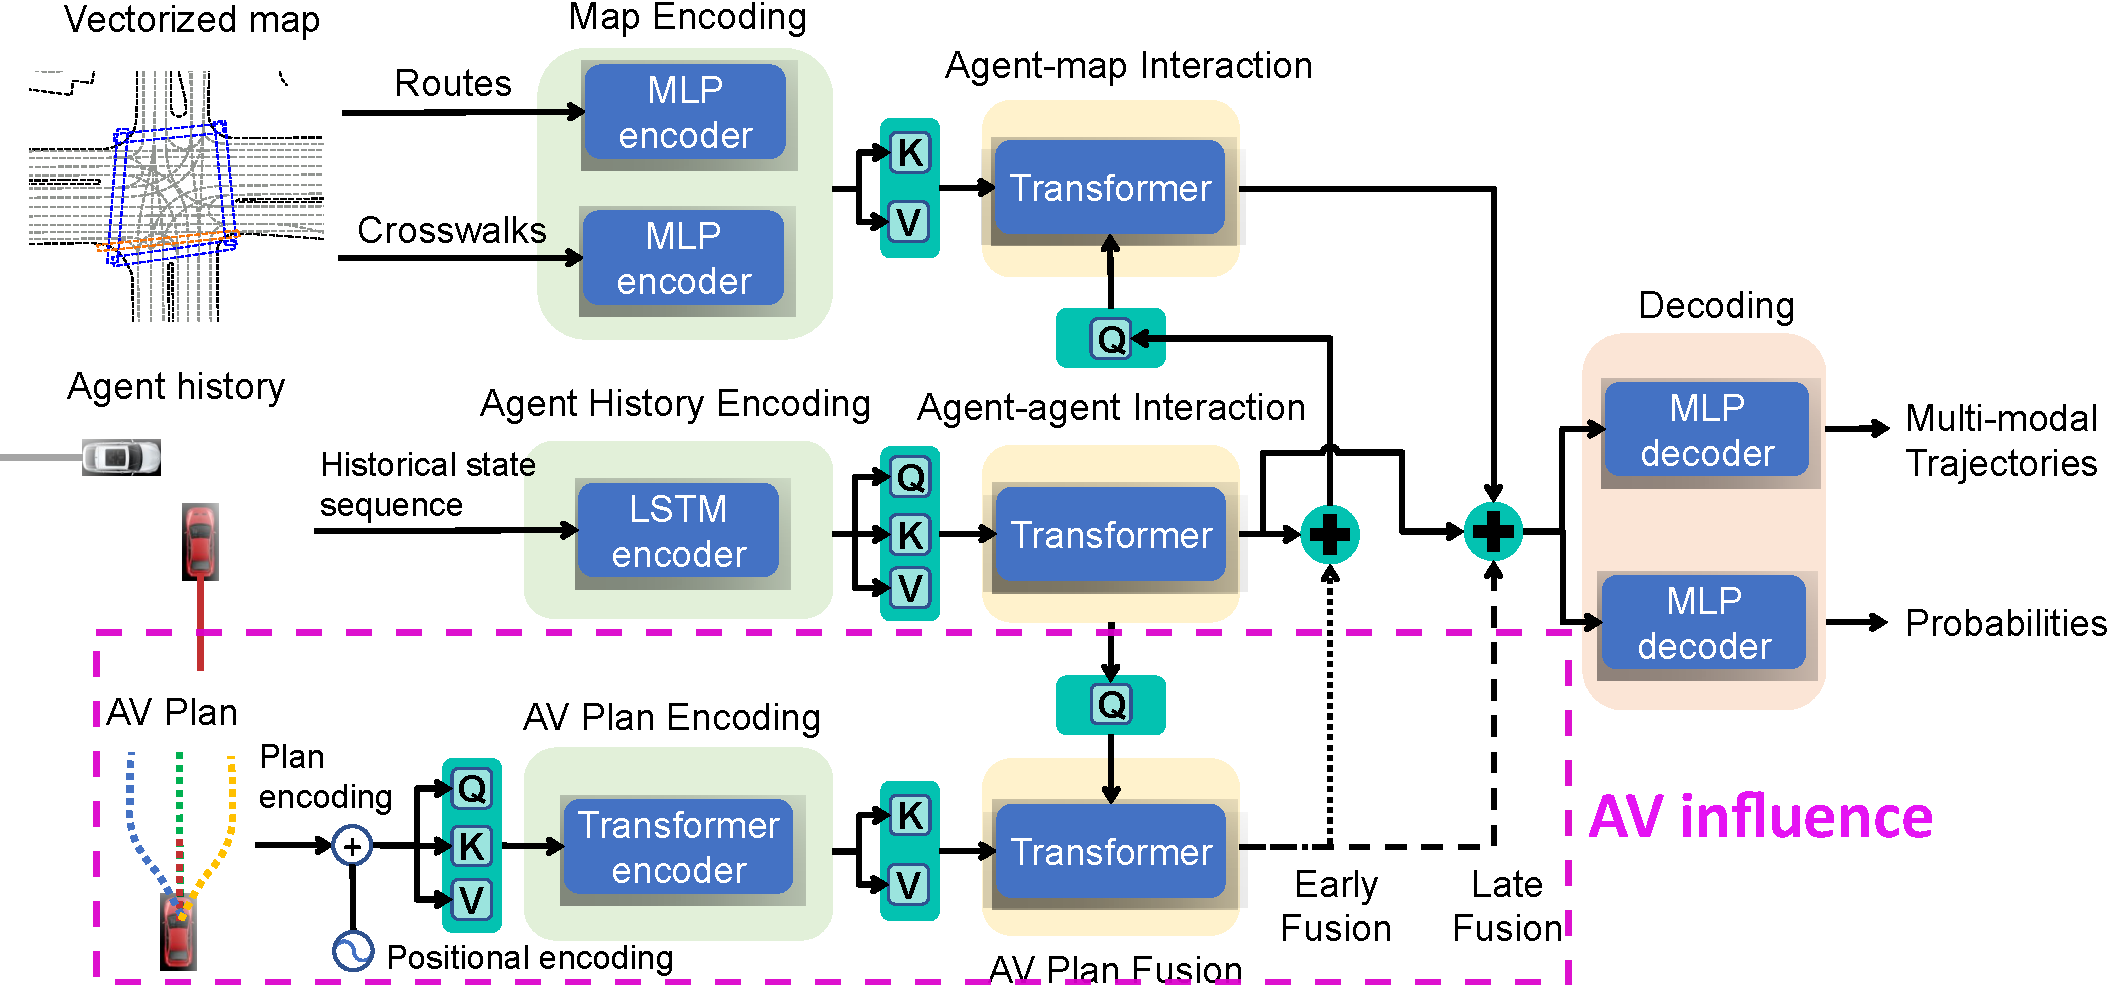
\includegraphics[width=\linewidth]{2_cmp_vs_pmp.pdf}
	\caption{Example of a Conditional Motion Prediction (CMP) network.} We \textcolor{magenta}{highlight} the influence of the \ac{AD} in the prediction of surrounding agents. \\
	Source: \textit{Conditional Predictive Behavior Planning with Inverse Reinforcement Learning for Human-like Autonomous Driving} \cite{huang2023conditional}
	\label{fig:2_cmp_vs_pmp}
\end{figure}

Nevertheless, to ensure safety under various predicted trajectories of the surrounding agents, our \ac{ADS} must overly conservative with inefficient maneuvers, specifically in arbitrarily complex traffic scenarios, because \ac{PMP} models ignore the fact that the future states of an agent can influence the future actions of other agents, what is the most realistic situation. To this end, researchers recently started to explore a more coherent interactive prediction and planning framework which relies on predicting the surrounding agents future trajectories conditioned on the ego-vehicle future actions \cite{tang2019multiple} \cite{rhinehart2019precog} \cite{khandelwal2020if}, as a preliminary state to implement a fully-interaction graph where the future states of all agents (either autonomous prototypes or human-driven) influence in the decision of all agents. Under such frameworks, the \acs{ADS} can reason over potential actions while considering its influence on surrounding agents, as observed in Figure \ref{fig:2_cmp_vs_pmp}, inducing less conservative and more efficient maneuvers in highly interactive scenarios. \cite{huang2023conditional} propose a learning-based behaviour planning framework that learns to predict conditional multi-agent future trajectories, evaluating decisions from real-world human data. Moreover, they propose a two-stage learning process where the prediction model is trained first conditioned on the \ac{ADS} future actions, and then used as an environment model in the learning of the cost function with maximum entropy Inverse Reinforcement Learning (IRL). \cite{tang2022interventional} argue that CMP-based models essentially learns the posterior distribution of future trajectories conditioned on the future states of the ego-vehicle, where this future trajectory is treated as an observation, whilst safe and realistic prediction models should build the \ac{MP} to approximate the future trajectory distribution under the intervention of enforcing the \ac{ADS} future states, referring this new task as Interventional Behaviour Prediction (IBP). As aforementioned, the algorithms studied and developed throughout this thesis do not focus on the joint study of the prediction and behaviour planning modules, but on building efficient and powerful \ac{PMP} algorithms without considering the future states of the autonomous agents as an additional condition. \\

Once the differences between \ac{CMP} and \ac{PMP} have been illustrated, we proceed with the problem formulation, main contextual factors and classification of prediction methods.

\section{Problem Formulation of Motion Prediction}
\label{sec:2_problem_formulation_mp}

Given a sequence of past trajectories $a_{P}=[a_{-obs_{len}^{'}+1},a_{-obs_{len}^{'}+2},...,a_{0}]$ for an agent, we aim to predict its future steps $a_{F}=[a_{1},a_{2},...,a_{pred_{len}}]$ up to a fixed time step $pred_{len}$. Running in a specific traffic scenario, each agent will interact with static HD maps $m$ and the other dynamic actors, meeting the corresponding traffic and social rules. Therefore, the probabilistic distribution that we want to capture is $p(a_F|m, a_P, a^O_P)$, where $a^O_P$ denotes the other agents observed states. The output of most existing methods is a set of trajectories $A_F = \{a_{F}^k\}_{k \in [0,K-1]}= \{(a_{1}^k,a_{2}^k,...,a_{pred_{len}}^k)\}_{k \in [0,K-1]}$ for each agent, where $K$ represents the number of modes or plausible future directions, due to the inherent uncertainty associated to the prediction problem. This set of trajectories for each agent will be used by downstream decision modules. On top of that, TNT (Target-driven trajectory prediction) \cite{zhao2021tnt} is one of the first methods that introduces specific preliminary future positions in the problem formulation, also referred as goals, being TNT \cite{zhao2021tnt}-like methods distribution approximated as:

\begin{equation}
	\sum_{\tau \in T(m, a_P, a^O_P)}{p(\tau|m, a_P, a^O_P)p(a_F|\tau, m, a_P, a^O_P)}
\end{equation}
where $T(m, a_P, a^O_P)$ is the space of candidate goals depending on the driving context.

However, the map space $m$ is large, and the goal space $T(m, a_P, a^O_P)$ requires careful design. In that sense, some methods expect to accurately predict the actor motion by extracting good features. For example, LaneGCN~\cite{liang2020learning} tries to approximate $p(a_F|m, a_P, a^O_P)$ by modeling $p(a_F|M_{a_0}, a_P, a^O_P)$, 
where $M_{a_0}$ is a "local" map features that is related to the actor's state $a_0$ at final observed step $t=0$.
To extract $M_{a_0}$, they use $a_0$ as an anchor to retrieve its surrounding map elements and aggregate their features. We found that not only the "local" map information is important, but also the goal area maps information is of great importance for accurate trajectory prediction. 
So, we reconstructed the probability as:

\begin{equation}
	\sum _{\tau}{p(\tau|M_{a_0}, a_P, a^O_P) p(M_{\tau}|m, \tau)p(a_F|M_{\tau},M_{a_0}, a_P, a^O_P)}
\end{equation}

We directly predict possible goals $\tau$ based on actors' motion histories and driving context. Therefore, GANet is genuinely end-to-end, adaptive, and efficient. 
Then, we apply the predicted goals as anchors to retrieve the map elements in goal areas explicitly and aggregate their map features as $M_{\tau}$.

\section{Contextual Factors and Classification of Motion Prediction methods}
\label{sec:2_contextual_factors_and_classification_mp}

This section studies the contextual factors (inputs) and classification of \ac{MP} in the field of \ac{AD} according to its encoding method of the different inputs and output types. Figure \ref{fig:2_input_output_mp} \cite{huang2022survey} summarizes the main inputs and outputs of these methods. \\

\begin{figure}[h]
	\centering
	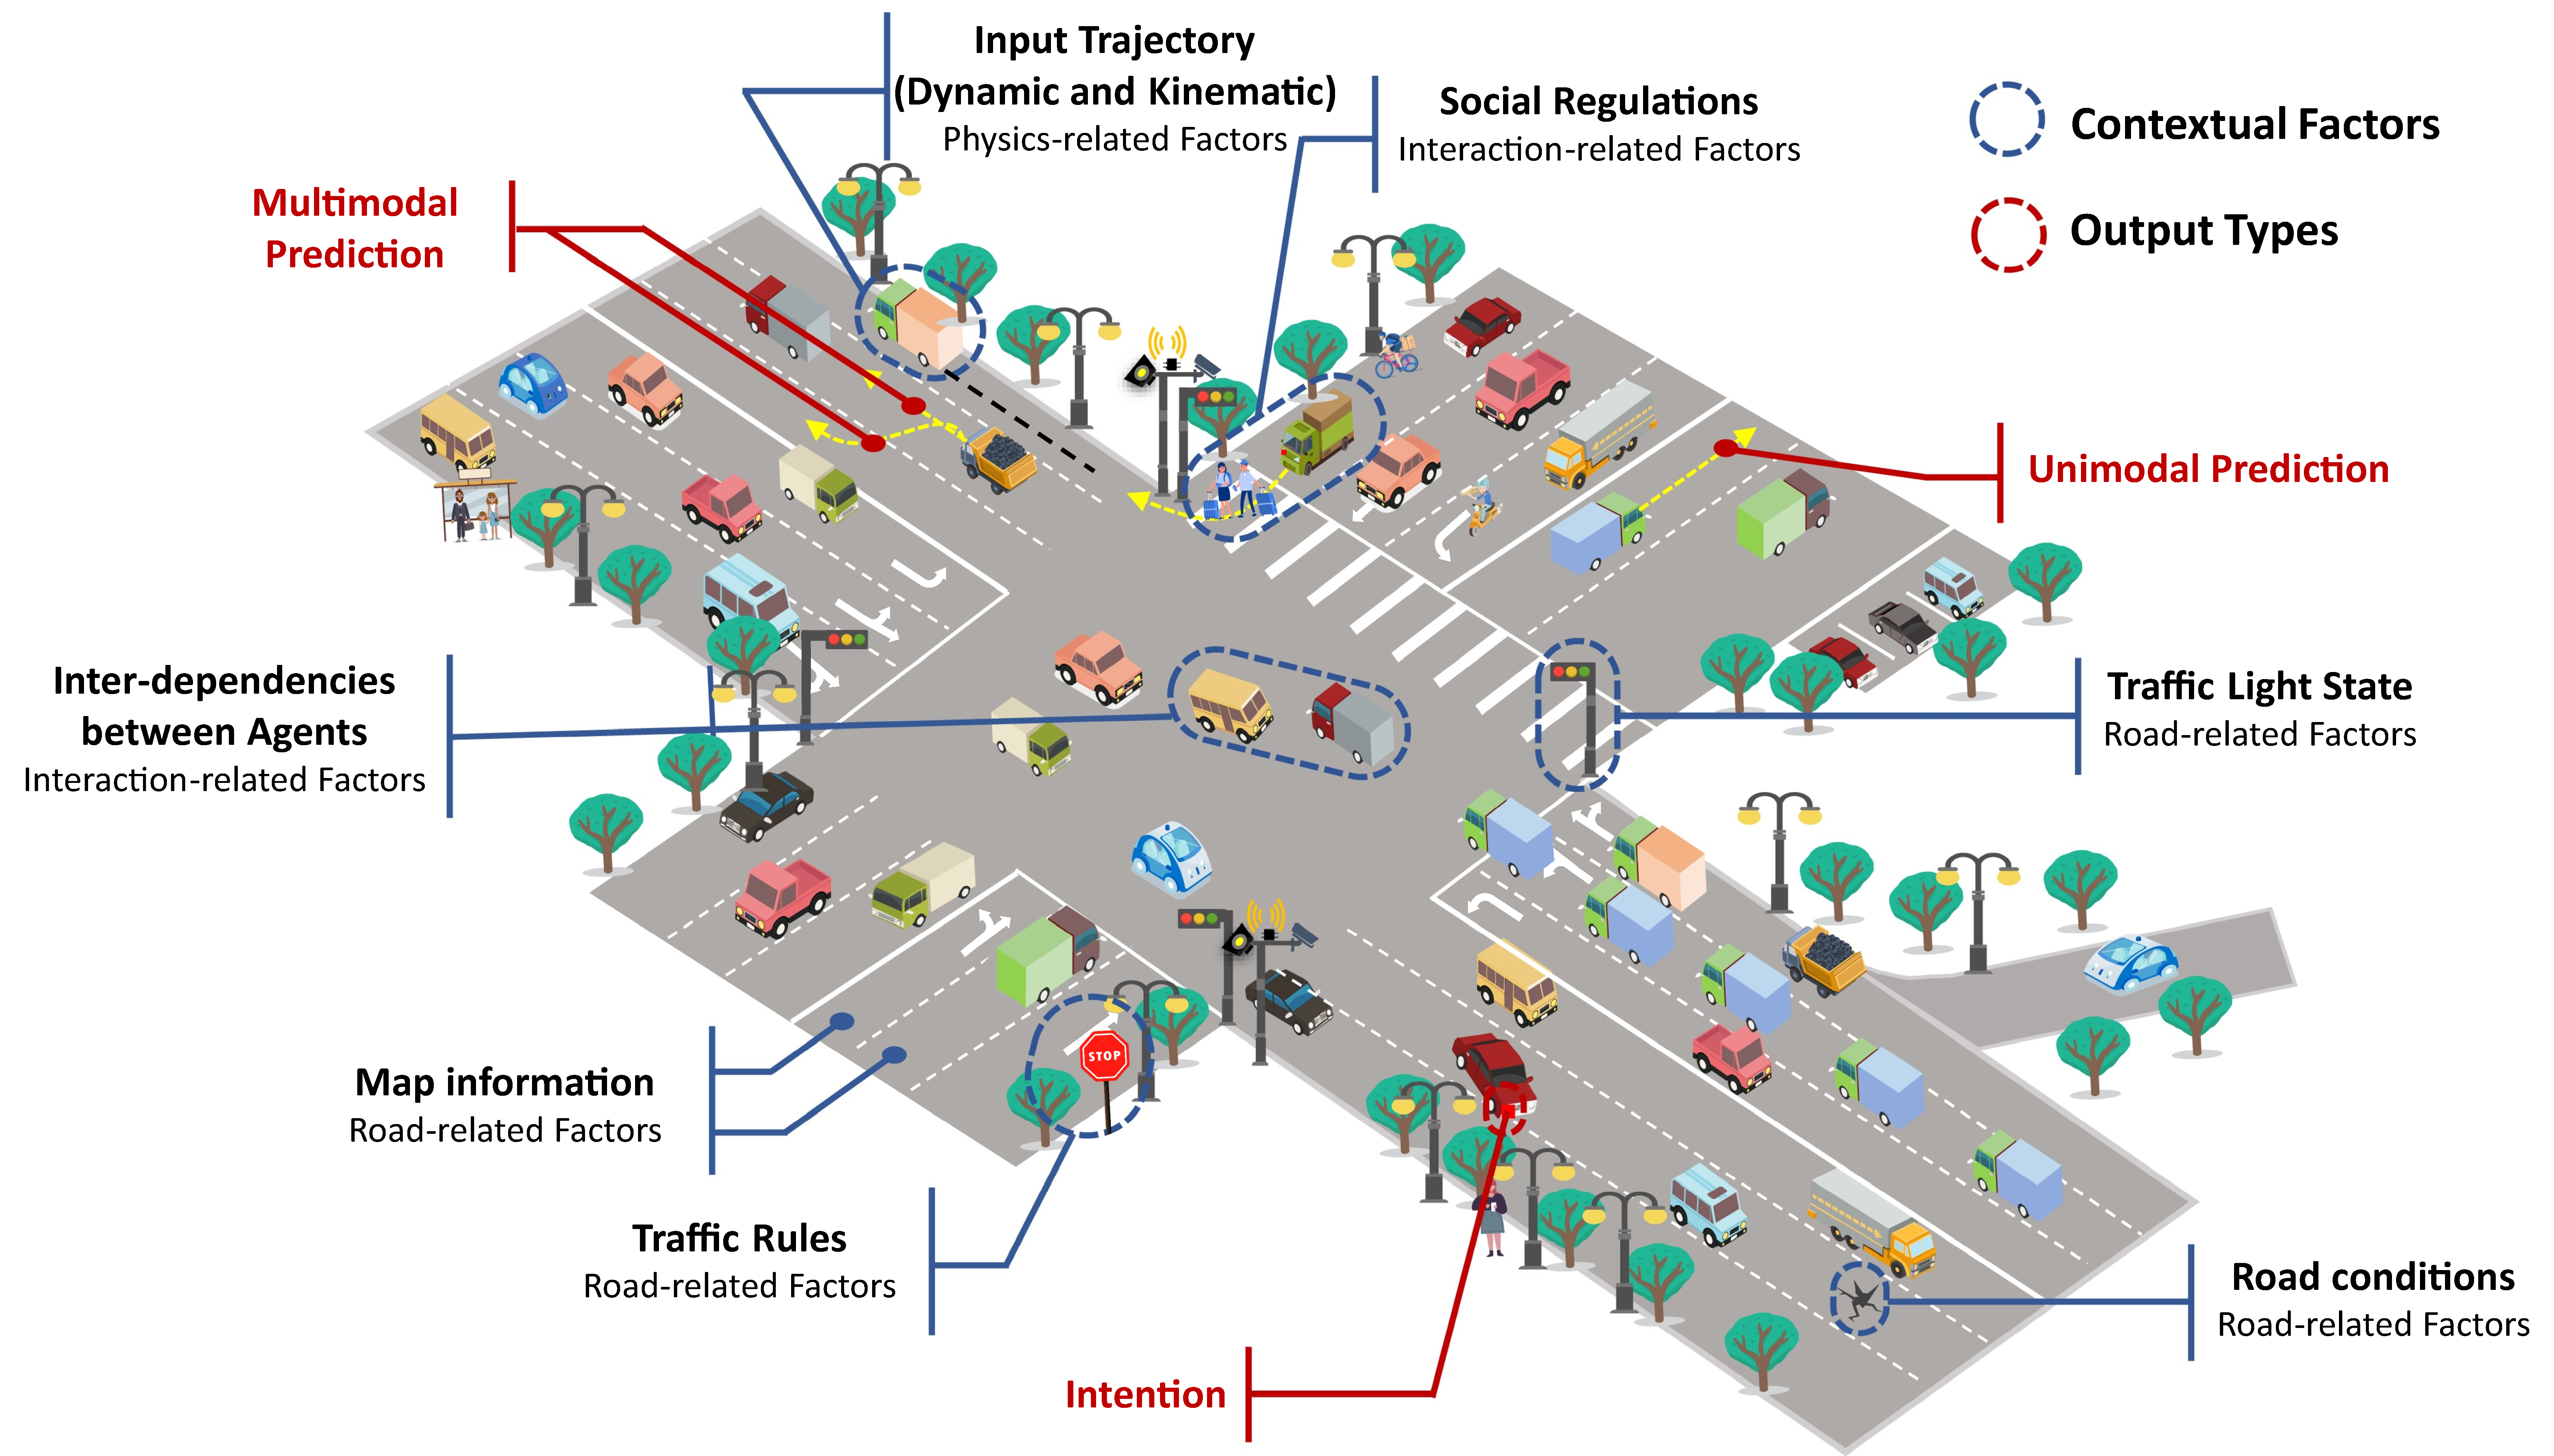
\includegraphics[width=\linewidth]{2_inputs_outputs_mp.pdf}
	\caption{Contextual factors and output types in Vehicle Motion Prediction}
	Source: \textit{A survey on trajectory-prediction methods for autonomous driving} \cite{huang2022survey}
	\label{fig:2_input_output_mp}
\end{figure}

In order to model the future states of surrounding agents, \ac{MP} models must pay attention to the current environment, where some contextual factors can be clearly identified:

\begin{itemize}
	\item Physics-related factors refer to the kinematic and dynamic variables of the agents, specifically to their spatio-temporal variables (such as position, velocity, acceleration, object type or mass) as well as past behaviours. 
	\item Interaction-related factors include the inter-dependencies and social regulations between agents maneuvers. It is important to consider that traffic agents can be either non-relevant pedestrians on the sidewalk as well as an extremely relevant truck in front of the ego-vehicle.
	\item Road-related factors include the corresponding traffic rules (lane type, traffic signals, stops, etc.) as well as the modeling
	of the map (usually HD-map), including its topological, semantic and geometrical information.
\end{itemize}

On the other hand, regarding the output types, \ac{MP} methods need to provide the future trajectories of traffic participants. Nevertheless, these methods can provide these future trajectories in different ways, even though these outputs can be unified as a single output, depending on the application:

\begin{itemize}
	\item Unimodal prediction. In the unimodal case, the prediction method only returns a single future trajectory, without taking into account other possible behaviours. 
	\item Multimodal prediction. Models that generate a multimodal prediction compute multiple \textit{K} future trajectories (also referred as modes in the literature) with the probability of each future trajectory. The higher the mode probability (also referred as score), the more probable this particular behaviour (turn left with a certain velocity and acceleration) should be. This output type is specially useful for fast-changing and highly interactive situations where multiple options are available. One important thing to note is that multimodal methods must be designed in order to not only reason in terms of different maneuvers (keep straight, turn right, lane change, etc.) but also different velocity profiles (constant velocity, acceleration, sudden break, etc.) regarding the same maneuver.
	\item Maneuver, also referred as intention, can be part of the final output or just be an intermediate step in the method. \ac{MP} methods usually produce maneuver intention to assist in the subsequent prediction.
\end{itemize}

As we will study throughout this section, most prediction methods focus on the multimodal output with an associated probability for each mode, since this is the most realistic way to imitate the human brain during navigation. First of all, there are plenty of problems during navigation, since there is a high uncertainty of traffic behavior and a large number of different situations. That means that one cannot use a discrete number of situations and a discrete number of car movements. Second, the main tasks of \ac{ADS}, like ensuring safe and efficient operations and anticipating a multitude of possible behaviors of traffic actors in its surroundings, provide a large need in knowing the position of all vehicles beforehand. Multimodal means that we have multiple predictions for each timeframe. Figure \ref{fig:2_um_vs_mm_mp} illustrates an interesting traffic scenario in the Argoverse 1 \cite{chang2019argoverse} Motion Forecasting dataset, processed by one our algorithms. The \textbf{\textcolor{YellowOrange}{target agent}} is getting close to an intersection, where several future maneuvers are plausible. In both cases (unimodal and multimodal, which are the most common ones), the model must reason the future trajectory of the target agent based on its past observations, interactions with other agents and physical context. On the left (\ref{fig:2_um_vs_mm_mp_a}) illustrates the unimodal case, where a single trajectory is predicted. On the right (\ref{fig:2_um_vs_mm_mp_b}), multiple trajectories (or modes) with associated probabilities are predicted, with most modes turning left and one mode keeping straight since in similar situations the agent could also perform this behaviour with a similar context. The main point of having this multimodality is to remove too generalized solutions. A lot of different algorithms study this problem, where quite similar inputs would produce similar predictions, while in reality this does not happens.

\begin{figure}[t!]
	\begin{subfigure}{0.5\textwidth}
		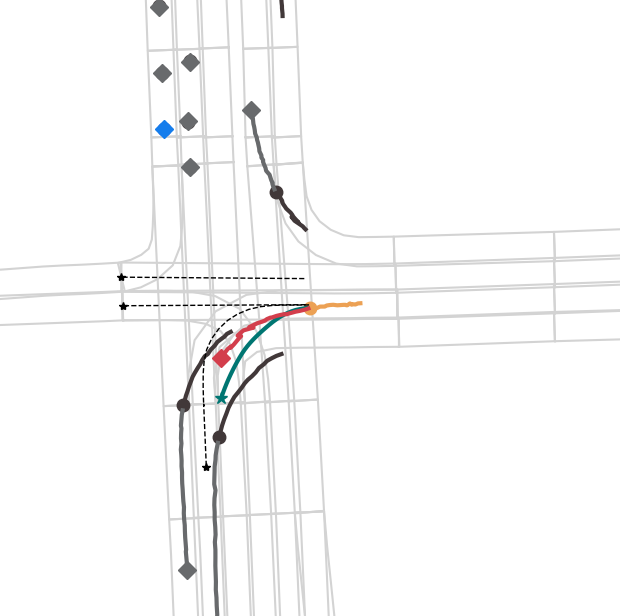
\includegraphics[width=\textwidth]{2_mm_example_um.png}
		\caption{Unimodal prediction}
		\label{fig:2_um_vs_mm_mp_a}
	\end{subfigure}
	\hfill
	\begin{subfigure}{0.5\textwidth}
		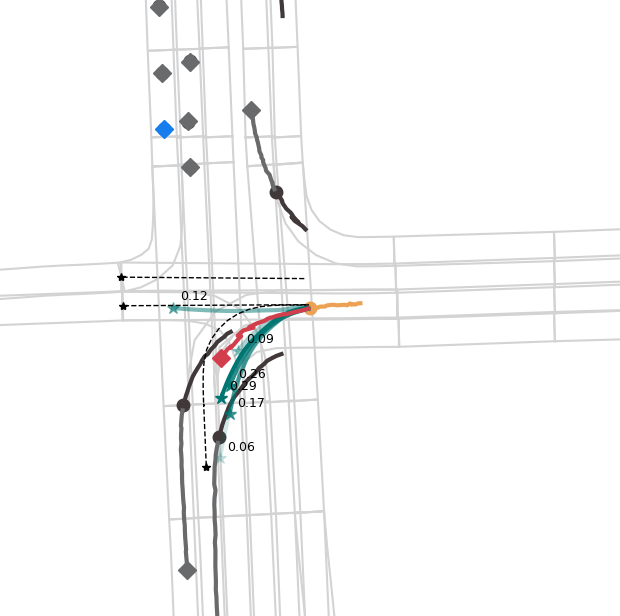
\includegraphics[width=\textwidth]{2_mm_example_mm.png}
		\caption{Multimodal prediction}
		\label{fig:2_um_vs_mm_mp_b}
	\end{subfigure}

	\caption[Modeling multimodality of future $3$-second agent trajectories with one of our algorithms]{Modeling multimodality of future $3$-second agent trajectories with one of our algorithms; We represent: our vehicle (\textbf{\textcolor{blue}{ego}}), the \textbf{\textcolor{YellowOrange}{target agent}}, and \textbf{\textcolor{gray}{other agents}}. We can also see the \textbf{\textcolor{red}{ground-truth}} trajectory of the target agent, our \textbf{\textcolor{ForestGreen}{multimodal predictions}} (with the corresponding confidences) and \textbf{plausible centerlines}. Circles represent last observations and diamonds last future positions.}
	\label{fig:2_um_vs_mm_mp}
\end{figure}

After defining the contextual factors and output types, a classification of the prediction methods according to different modeling approaches is illustrates. Over the last two decades, \ac{MP} can be divided into four parts in chronological order: Physics-based, classic Machine Learning-based, Reinforcement Learning-based and Deep Learning-based, as shown in Figure \ref{fig:2_taxonomy_mp}. The remaining content of this section, based on the study performed by \cite{huang2022survey}, illustrates the main algorithms used in each part, especially focusing on \ac{DL} since in this work we focus on predictive techniques for scene understanding based on deep models.

\begin{figure}[h]
	\centering
	% trim={left bottom right top}
	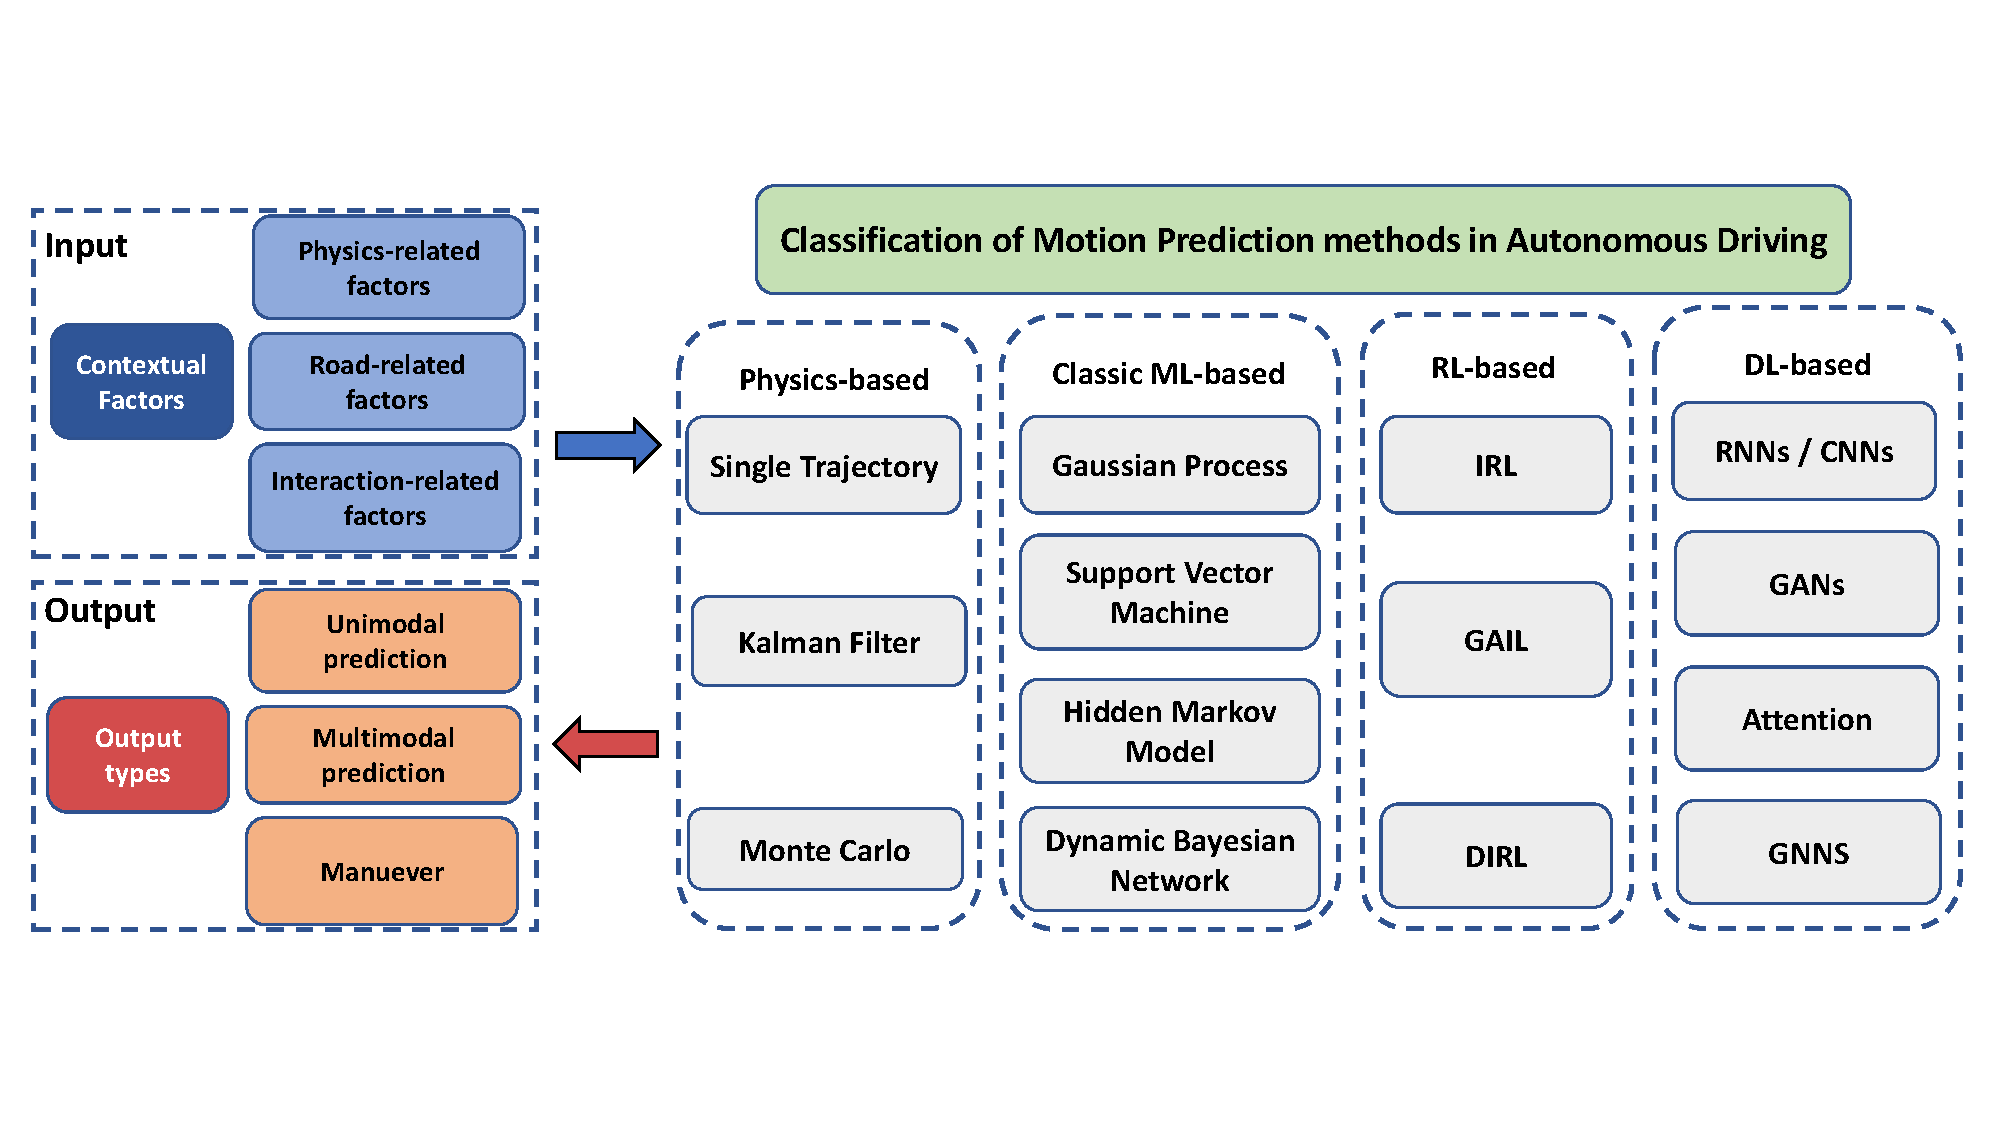
\includegraphics[trim={0 1cm 0 1cm}, width=\linewidth]{2_taxonomy_mp.pdf}
	\caption{Contextual factors and output types in Vehicle Motion Prediction}
	%Source: \textit{A survey on trajectory-prediction methods for autonomous driving} \cite{huang2022survey}
	\label{fig:2_taxonomy_mp}
\end{figure}

\subsection{Physics-based Motion Prediction}
\label{subsec:2_physics_based_mp}

Physics-based methods are the first and simplest methods used by researchers. Although the accuracy of these methods is relatively low, more and more models use the idea of physics-based models to improve the accuracy. Physics-based methods have more accurate results when the movement of vehicles can be accurately described by kinematics or dynamics models, but the physical model of the traffic participants is constantly changing, such that most of these methods are only suitable for short-term prediction (no more than 1-s). Dynamics models can be quite complex, including many inherent parameters and introducing an extra computation burden, in such a way that researchers prefer simple dynamic methods for motion prediction. In terms of vehicle \ac{MP}, the bicycle model is usually employed to model the vehicle physics, driven by the front wheels \cite{kaempchen2009situation, pepy2006reducing}. In the literature three main types of physics-based models are distinguished, where the main different is the way in which the uncertainty is handled: Single Trajectory, Kalman Filter-based and Monte Carlo-based.

\subsubsection{Single-Trajectory}
\label{subsubsec:2_single_trajectory_mp}

One of the most straightforward methods to predict an agent trajectory is to directly apply the agent current state to the physic model. In order to increase the accuracy and stability of the estimation, the vehicles are mostly assumed to comply with motion models that describe their dynamic behavior. In the past, numerous motion models (with different degrees of complexity) have been proposed for this task \cite{miller2002adaptive, pepy2006reducing, hillenbrand2006multilevel}. A first systematization can be achieved by defining different levels of complexity. At the lower end of such a scale, linear motion models are situated. These models assume a Constant Velocity (CV) or a Constant Acceleration (CA). Their major advantage is the linearity of the state transition equation which allows an optimal propagation of the state probability distribution. On the other hand, these models assume straight motions and are thus not able to take rotations (especially the yaw rate) into account. \\

A second level of complexity can be defined by taking rotations around the $z$-axis into account. The resulting models are sometimes referred to as curvilinear models. They can be further divided by the state variables which are assumed to be constant. The most simple model of this level is the Constant Turn Rate and Velocity (CTRV) model. By defining the derivative of the velocity as the constant variable, the Constant Turn Rate and Acceleration (CTRA) model can be derived. Both CTRV and CTRA assume that there is no correlation between the velocity $v$ and the yaw rate $\omega$. As a consequence, disturbed yaw rate measurements can change the yaw angle of the vehicle even if it is not moving. \\

In order to avoid this problem, the correlation between $v$ and $\omega$ can be modeled by using the steering angle $\Phi$ (angle between the axis of motion and the direction of the front wheels) as constant variable and derive the yaw rate from $v$ and $\Phi$. The resulting model is called Constant Steering Angle and Velocity (CSAV). Again, the velocity can be assumed to change linearly, which leads to the Constant Curvature and Acceleration (CCA) model. \\

From a geometrical point of view, nearly all curvilinear models are assuming that the vehicle is moving on a circular trajectory (either with a constant velocity or acceleration). The only exception is the CTRA model which models a linear variation of the curvature and thus assumes that the vehicle is following a clothoid. \\

While in theory curvilinear models describe the motion of road vehicles very accurately, errors may result from highly dynamic effects such as drifting or skidding. While models which are able to cope with such effects do exist, they will not be considered here for two reasons: Firstly, most \ac{ITS} applications are designed for scenarios with non-critical dynamics. Secondly, the required information for estimating the additional parameters (e.g. slip from every tire, lateral acceleration) are not observable by exteroceptive sensors. Furthermore, these methods are not able to consider the road-related factors and the uncertainty of the current state is unreliable for long-term prediction in such a way these single trajectory models should only be used for estimating unimodal trajectories of the surrounding agents in the short-term. We further study the state transition equations of physics-based models in Chapter \ref{cha:theoretical_background} since they will be used in the algorithms proposed in this thesis as preliminary proposals for the \ac{DL} models.

\subsubsection{Kalman Filter}
\label{subsubsec:2_kalman_filter_mp}

Kalman Filter (KF)-based methods aim to solve one of drawbacks of physics-based models: In real-world, the states of agents are not perfectly known since they present an associated noise. KF-based methods model the uncertainty oir noise of the current agent state and its physic model by means of a Normal (Gaussian) distribution. Compared to the single trajectory methods, the main advantage is that KF methods consider the uncertainty of the predicted trajectory, specially when using its Extended (EKF) or Unscented (UKF) where non-linearities can be modeled. As proposed by the original algorithm \cite{kalman1960new}, the prediction and update steps are combined into a loop where the mean value and covariance matrix of the agent state is computed for each future step, calculated as an average trajectory with related uncertainty. \\

Nevertheless, these KF-based methods are unimodal Gaussian distributions which are not enough to represent agents interactions. In that sense, \cite{kaempchen2004imm} propose an Interactive Multiple Model (IMM) to compute a multimodal prediction. Moreover, \cite{jin2015switched} model a set of Kalman Filters used to describe physical models of the vehicles and switch between them, defined as Switched Kalman Filter (SKF). \cite{lefkopoulos2020interaction} propose IMM-KF, a novel Interacting Multiple Model Kalman Filter which takes interaction-related factors (social regulation, inter-dependencies) into consideration, as shown in Figure \ref{fig:2_input_output_mp}.

\subsubsection{Monte Carlo}
\label{subsubsec:2_monte_carlo_mp}

In the same way KF methods aimed to solve the associated noise to the physics state of the agent, Monte Carlo method aims to simulate the state distribution approximately since an analytical expression for the predicted state distribution is usually unknown without any assumptions of the linearity or the model’s Gaussian nature. This method randomly samples the input variables and applies the physics model to compute potential future trajectories. In order to ensure the plausibility of the future behaviour in the context of \ac{AD}, the generated future states are usually filtered with a lateral acceleration lower than the actual allowable lateral acceleration \cite{broadhurst2005monte}, though other vehicle physical limitation can also be used such that the input of the model will be more realistic. \cite{okamoto2017driver} present a model that identifies a preliminary maneuver and then applies the Monte Carlo method to compute future trajectories by the identified maneuver. Furthermore, \cite{wang2019trajectory} first use the Monte Carlo algorithm to predict future trajectories and then utilize MPC (Model Predictive Control) algorithm to refine these preliminary future trajectories.

\subsection{Classic Machine Learning based Motion Prediction}
\label{sec:2_ml_based_mp}

Classic ML \ac{MP} methods make use of data-driven models to predict trajectories instead of only considering the physical model. These methods determine the probability distribution by mining data features. These methods provide new ideas for \ac{MP}, which promote the development of learning-based approaches. With more factors to be considered, the accuracy of these methods keeps increasing, being most of them maneuver-based (which is provided or identified in advance) in order to subsequently estimate the future states of the agents by first judging the corresponding maneuver. Regarding the field of vehicle \ac{MP}, we can find in the literature four main types of classic ML methods: Gaussian Process, Support Vector Machine (SVM), Hidden Markov Model (HMM) and Dynamic Bayesian (Network). Figure \ref{fig:2_dbn_mp} illustrates some these methods. 

\begin{figure}[t!]
	\begin{subfigure}{0.5\textwidth}
		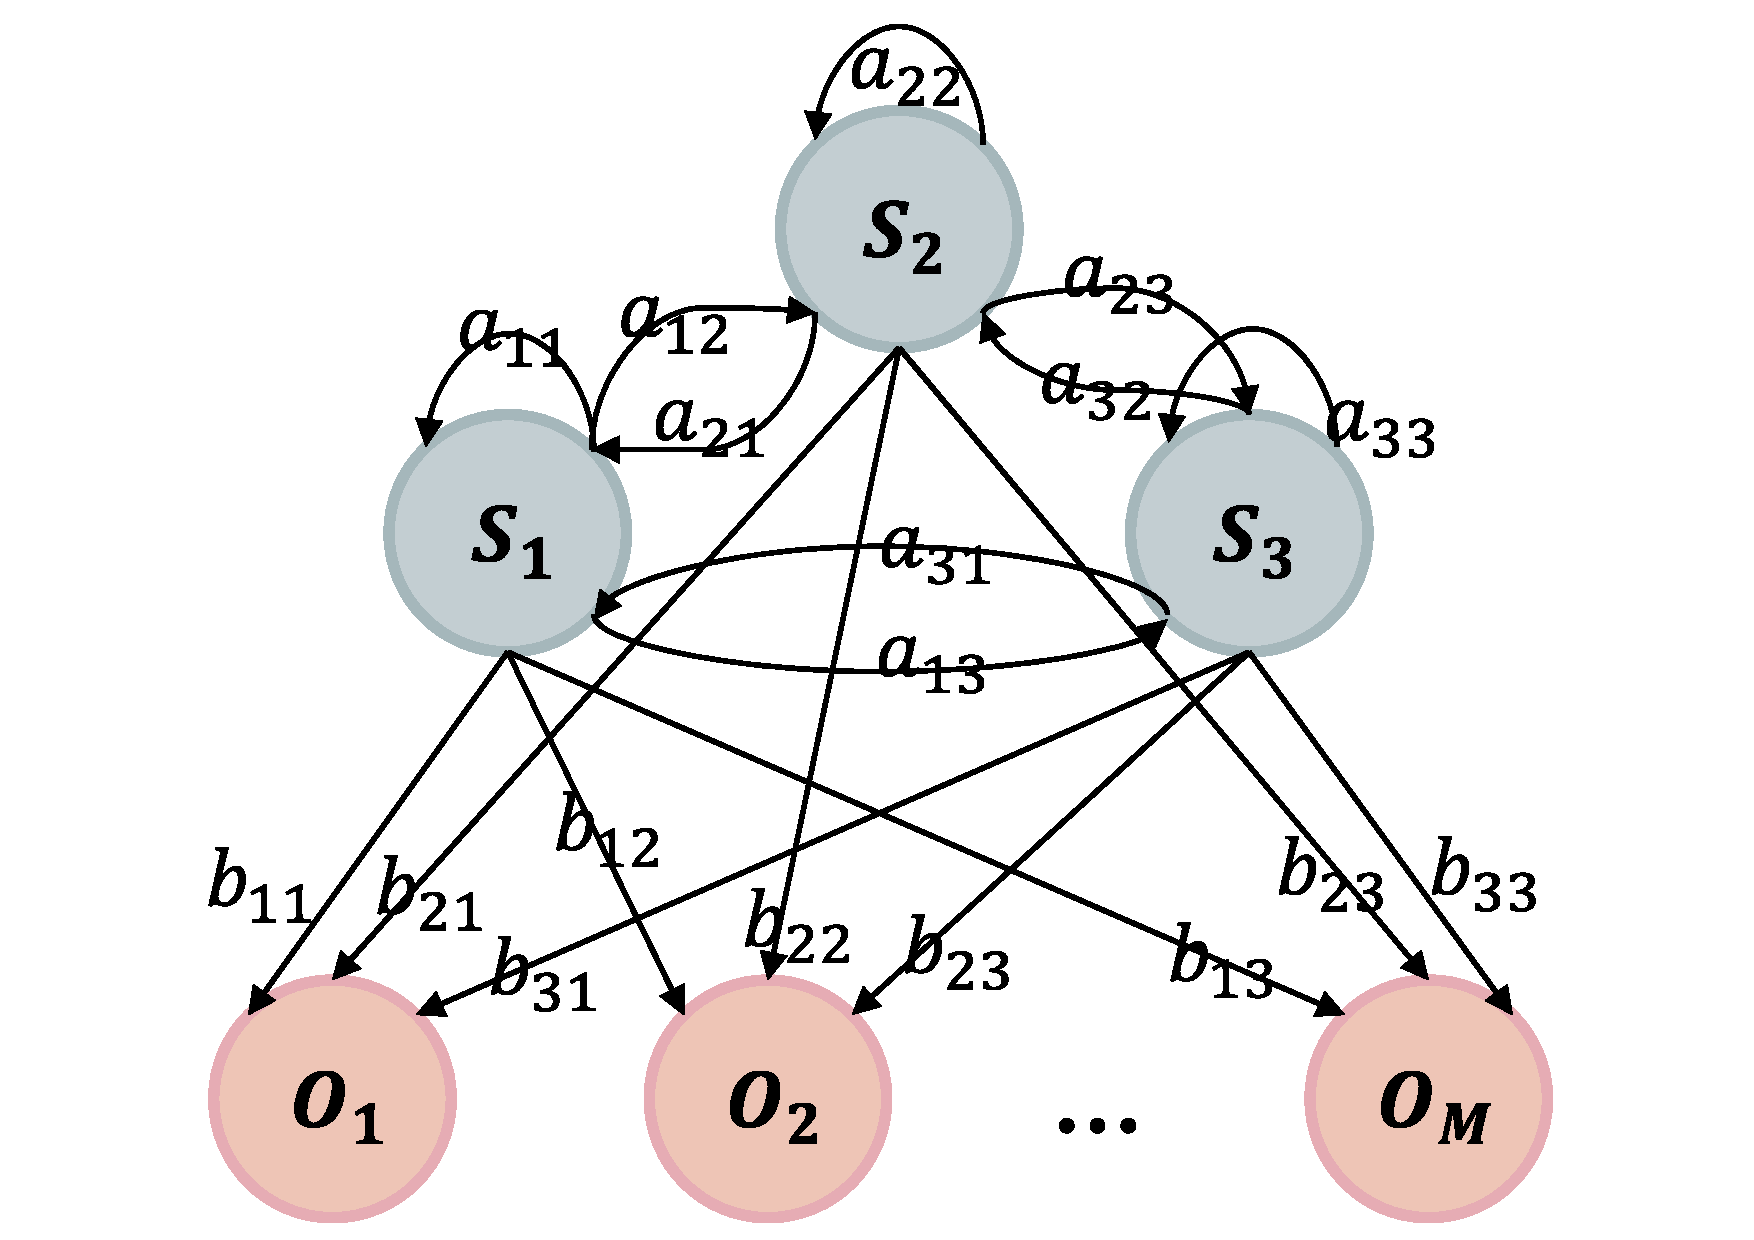
\includegraphics[width=\textwidth]{2_hmm_mp.pdf}
		\caption{Hidden Markov Model}
		\label{fig:2_hmm_mp}
	\end{subfigure}
	\hfill
	\begin{subfigure}{0.5\textwidth}
		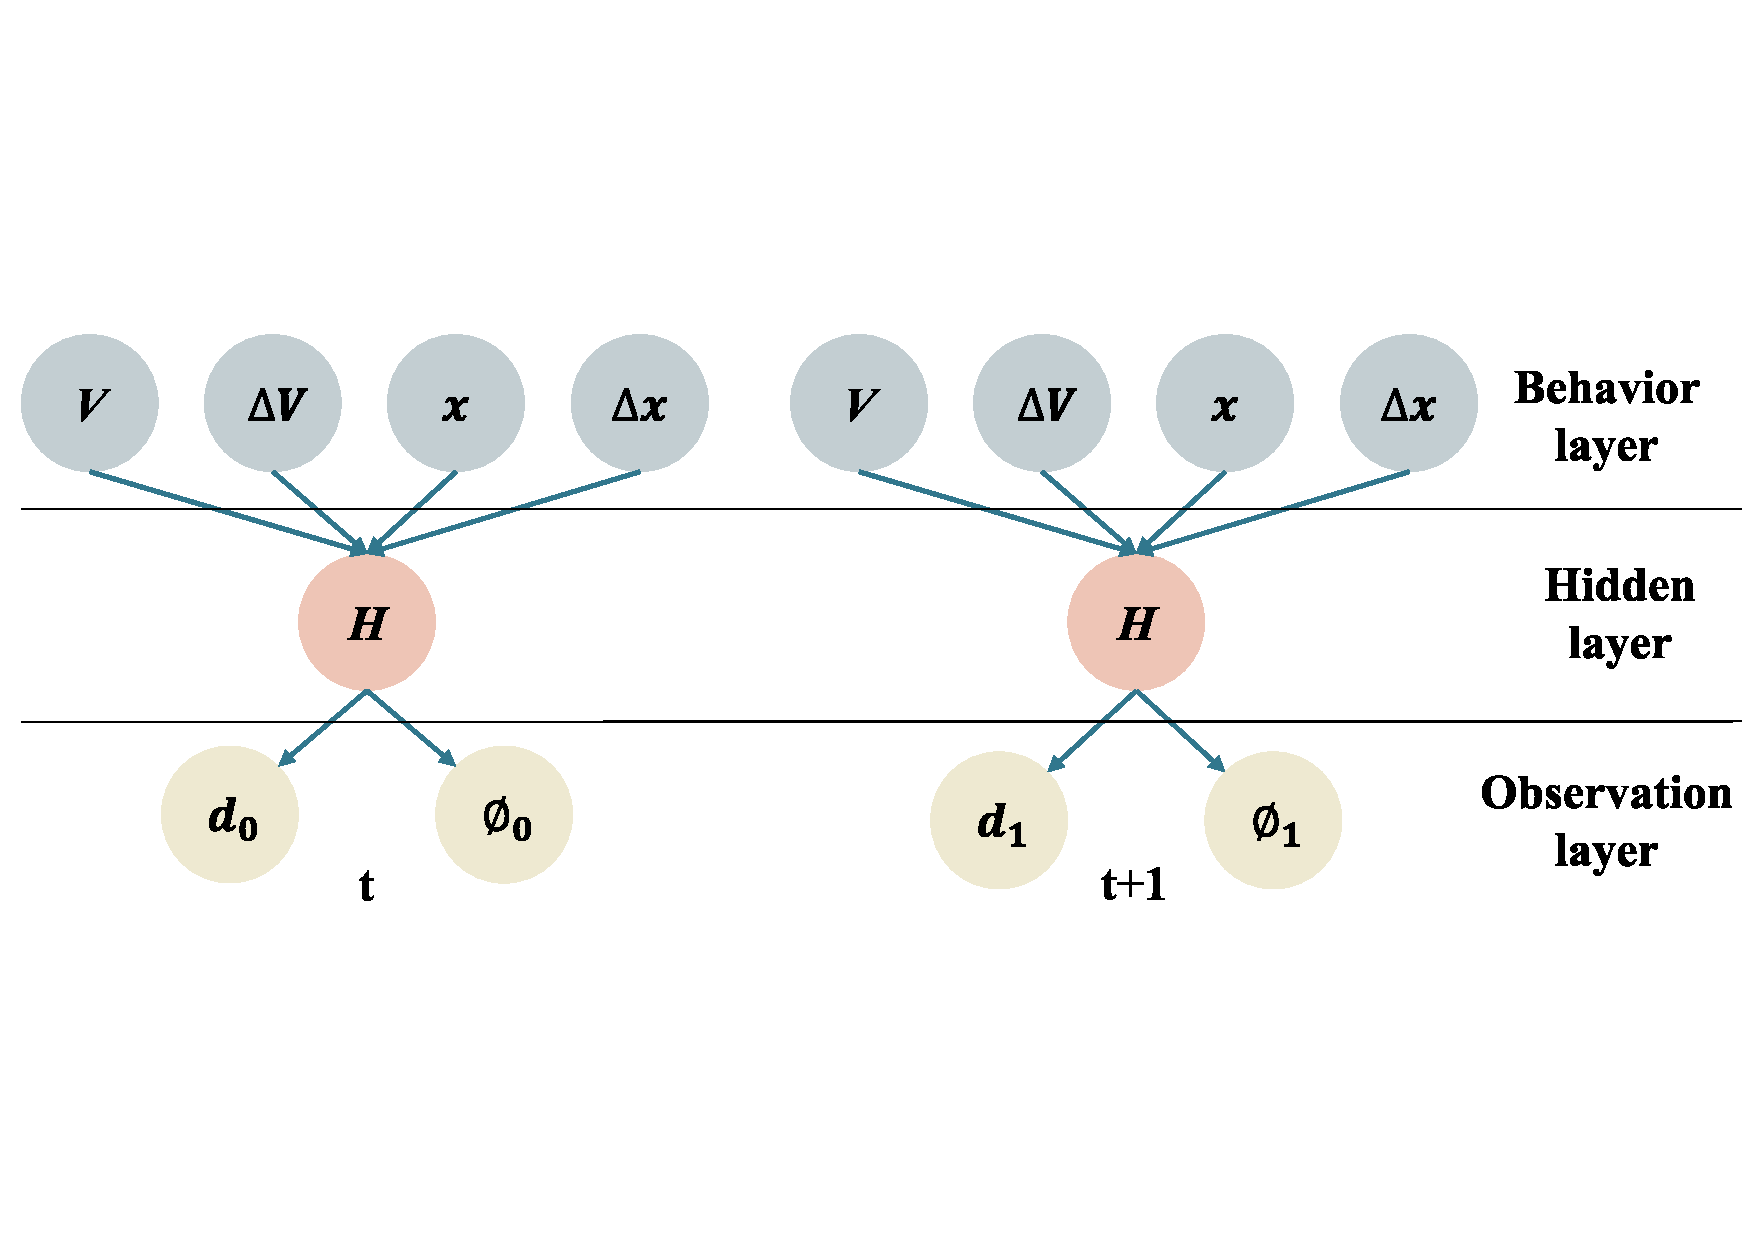
\includegraphics[width=\textwidth]{2_dbn_mp.pdf}
		\caption{Dynamic Bayesian Network}
		\label{fig:2_dbn_mp}
	\end{subfigure}
	
	\caption[Some typical Classic Machine Learning algorithms in Motion Prediction]{Some typical Classic Machine Learning algorithms in Motion Prediction, like Hidden Markov Model and Dynamic Bayesian Network.}
	Source (a): \textit{Improved driving behaviors prediction based on fuzzy logic-hidden markov model (fl-hmm)} \cite{deng2018improved} \\
	Source (b): \textit{Probabilistic intention prediction and trajectory generation based on dynamic bayesian networks} \cite{he2019probabilistic}
	\label{fig:2_classic_ml_mp}
\end{figure}

\subsubsection{Gaussian Process}
\label{subsubsec:2_gaussian_process_mp}

Gaussian Process (GP) applied in ML \cite{rasmussen2004gaussian} is identified as an stochastic process (collection of random variables indexed time or space) such that every finite collection of those random variables has a multivariate normal distribution, i.e. every finite linear combination of them is normally distributed. This stochastic process may be used to solve the prototype trajectory method \cite{joseph2011bayesian, tran2014online}, which a maneuver-based method that divides agents trajectories into a collection of several types of prototype trajectories. First, past trajectories are regarded as the samples of the GP, sampled along the time axis, being these samples represented by \textit{N} discrete points to map the \textit{N}-dimensional space, which is equivalent to satisfy the \textit{N}-dimensional Gaussian distribution. Therefore, the main task of the GP model regarding the prototype trajectory method is to determine the parameters of GP through the samples. Once these parameters have been obtained by means of the stochastic, the prototype trajectory method measures the similarity between the input historical trajectory and the computed prototype set to predict the most plausible future motion. GP can also be used to model interaction-related factors, as shown in Figure \ref{fig:2_input_output_mp}. \cite{trautman2010unfreezing} solve the frozen robot problem, where the environment surpasses a certain level of complexity and the robot planner decides to freeze in place to avoid collisions, by means of GP for joint collision avoidance. Furthermore, \cite{guo2019modeling} apply GP and Dirichlet Process (DP) to define motion processes and apply a non-parametric Bayesian network to extract potential motion patterns.

\subsubsection{Support Vector Machine (SVM)}
\label{subsubsec:2_svm_mp}

Support Vector Machine (SVM) increases the level of complexity over previous methods, being able to learn and recognize an agent maneuver in a complex environment. The main idea of SVM is to find the support vector that meets the classification requirements and determine the optimal hyperplane which can maximize the interval of the classified data. In particular, when applied to the \ac{MP} problem in \ac{AD}, driving maneuvers are usually classified into several categories: keep straight, turn left, turn right, break, etc. In that sense, it uses the kernel function to convert the input data to high-dimensional and perform linear classification in the space to identify the current driving maneuvers so as to predict the future steps. \cite{mandalia2005using} apply SVM to identify a lane changing maneuver, using the position, velocity, acceleration and steering wheel angle of the corresponding vehicle as input features for identification. \cite{kumar2013learning} propose a layered architecture method combining SVM and Bayesian filtering to identify lane-changing maneuvers so as to obtain more accurate identification results. Furthermore, \cite{aoude2009using} make use of SVM to identify the maneuvers of traffic participants. Nevertheless, according to the SVM definition which output the characteristics of classification probability, the user must present the categories or possible maneuvers in advance which will will also impact the final prediction results.

\subsubsection{Hidden Markov Model (HMM)}
\label{subsubsec:2_hmm_mp}

As aforementioned, SVM can be effective in classification problems, but in the field of \ac{MP} in \ac{AD} not as effective as a Hidden Markov Model (HMM). This is one of the most popular maneuver-based classic ML \ac{MP} methods, which uses Markov Chain. The Markov Chain refers to a stochastic process describing a sequence of possible events in which the probability of each event depends only on the state attained in the previous event, i.e. , the state at time $t+1$ of the system is only related to the previous time $t$, and the state transition probability is not related to time. Figure \ref{fig:2_hmm_mp} illustrates this model. The mathematical expression is:

\begin{equation}
	\begin{aligned}
		\mathrm{P}\left(S_{n+1}\right. & \left.=s \mid S_1=s_1, S_2=s_2 \cdots, S_n=s_n\right) \\
		& =\mathrm{P}\left(S_{n+1}=s \mid S_n=s_n\right) .
	\end{aligned}
\end{equation}

In real life, we can only observe the distinct state that is exposed on the surface, but no intuitive representation of its hidden states exists. Therefore, it is necessary to establish a Markov process with hidden states and get the essential states of events through the observable states set related to the hidden states probability, which is the so-called Hidden Markov Model. HMM is represented by $(S, O, A, B, \pi)[50]$, as shown in Figure \ref{fig:2_hmm_mp}:

\begin{itemize}
	\item $S=\left\{S_1, S_2, \cdots S_N\right\}$ represents the hidden states sequence
	\item $O=\left\{O_1, O_2, \cdots O_M\right\}$ represents the observation sequence
	\item $A$ represents the transition probability matrix between hidden states
	\item $B$ is the output matrix, representing the transition probability of hidden states to output states
	\item $\pi$ is the initial probability matrix, representing the initial probability distribution in hidden states
\end{itemize}

When HMM is used in the trajectory prediction, the historical states of traffic participants are represented by observation sequence $O$, and HMM solves the most likely future observation sequence. \cite{deng2018improved} combine HMM with Fuzzy Logic for driver maneuver prediction. In \cite{wang2021decision}, HMM is used for trajectory prediction and risk assessment, and the results of are fed into the decision-making and planning system. Although traditional HMM methods have achieved a great success in predicting driver’s maneuvers, they do not consider the impact of interaction-related factors in the prediction process, such that its prediction results are not accurate enough in actual traffic scenes. To solve this issue, \cite{deo2018would} propose a vehicle trajectory prediction model based on HMM and Variational Gaussian Mixture Models (GMM) considering interaction-related factors. The vehicle interaction information is obtained by finding the optimal solution of the energy function.

\subsubsection{Dynamic Bayesian Network (DBN)}
\label{subsubsec:2_dbn_mp}

Dynamic Bayesian Networks (DBNs) \cite{koller2009probabilistic} solve the aforementioned issue of HMM when modeling the inter-dependencies among traffic participants, since in order to improve the accuracy of \ac{MP}, the prediction model should consider at least both vehicle states and the interaction effect between traffic participants. While Bayesian Networks describe static systems, DBNs introduce the concept of time segments to solve timing issues in probabilistic models. Time segment refers to a time template materialized according to DBN, which discretizes continuous time into countable points with preset time granularity. \\

Generally, the preset time granularity should be consistent with the actual state acquisition frequency, and DBN is trained according to the sensor sampling frequency as the time segment. Besides, the inference and learning methods of DBN need to be converted into Bayesian Networks before they can be directly applied. The architecture of DBN includes a behavior layer, a hidden layer, and an observation layer, as shown in Figure \ref{fig:2_dbn_mp}. The behavior layer represents the network input information, and the observation layer represents the driver’s maneuver. DBN models the effect of interaction between traffic participants when applied to trajectory prediction and perform well in classic machine learning-based methods. Using this architecture, Gindele et al. [59] model the driving maneuvers of multiple vehicles. The input information includes all vehicle states, vehicle interaction relationships, road structures, observation states, etc. \cite{schreier2016integrated} apply DBN to judge driving maneuvers and utilize the kinematics model corresponding to each driving maneuver to predict the trajectory. In \cite{bahram2015game}, the vehicle maneuver is predicted by game theory, and then the vehicle motion is judged by DBN which considers the interaction-related factors. In \cite{li2019dynamic}, DBN is designed to consider physics-related factors, road-related factors, and interaction-related factors. As maneuver-based methods, DBN models obtain high recognition performance and have been used in several real-world tests \cite{weidl2014optimizing}. However, DBN still faces the error problem from recognizing maneuvers to generating trajectories. Many methods can only judge two or three maneuvers, such as lane-keeping and lane-changing, and the model’s generalization ability is not strong.

\subsection{Reinforcement Learning based Motion Prediction}
\label{sec:2_rl_based_mp}

Reinforcement learning (RL) is one of three basic ML paradigms, alongside supervised learning and unsupervised learning. RL is an area of machine learning concerned with how intelligent agents ought to take actions in an environment in order to maximize the notion of cumulative reward. When RL is used in the field of \ac{MP} for \ac{AD}, most methods use the Markov decision process (MDP) to maximize the expected cumulative reward and generate optimal driving policies by learning expert demonstrations, most of which are planning-based methods. A MDP is a tuple $(\boldsymbol{S}, \boldsymbol{A}, \boldsymbol{P}, \boldsymbol{R}, \gamma)$, where $\boldsymbol{S}$ is a finite set of states, $\boldsymbol{A}$ is a finite set of actions, $\boldsymbol{P}$ is a state transition probability matrix, $P_{s s^{\prime}}^a=\mathbb{P}\left[S_{t+1}=s^{\prime}\right.$ $\left.S_t=s, A_t=a\right], \boldsymbol{R}$ is a reward function, $R_s^{\mathrm{a}}=\mathbb{E}\left[R_{t+1} \mid S_t=\right.$ $\left.s, A_t=a\right]$, and $\gamma$ is a discount factor. To find the best decision process over all policies, the optimal state-value function $v_{\star}(s)$ and the optimal action-value function $q_{\star}(s, a)$ can be calculated as:

\begin{equation}
\begin{aligned}
	v_*(s) & =\max _a\left[R_s^a+\gamma \sum_{s^{\prime} \in A} P_{s s^{\prime}}^a v_*\left(s^{\prime}\right)\right], \\
	q_*(s, a) & =R_s^a+\gamma \sum_{s^{\prime} \in A} P_{s s^{\prime}}^a \max _{a^{\prime}} q_*\left(s^{\prime}, a^{\prime}\right) .
\end{aligned}
\end{equation}

Using MDP, the RL-based methods can be classified as Inverse Reinforcement Learning (IRL) methods, Generative Adversarial Imitation Learning (GAIL) methods, and Deep IRL (DIRL) methods, which will be discussed below.

\begin{figure}[t!]
	\begin{subfigure}{0.5\textwidth}
		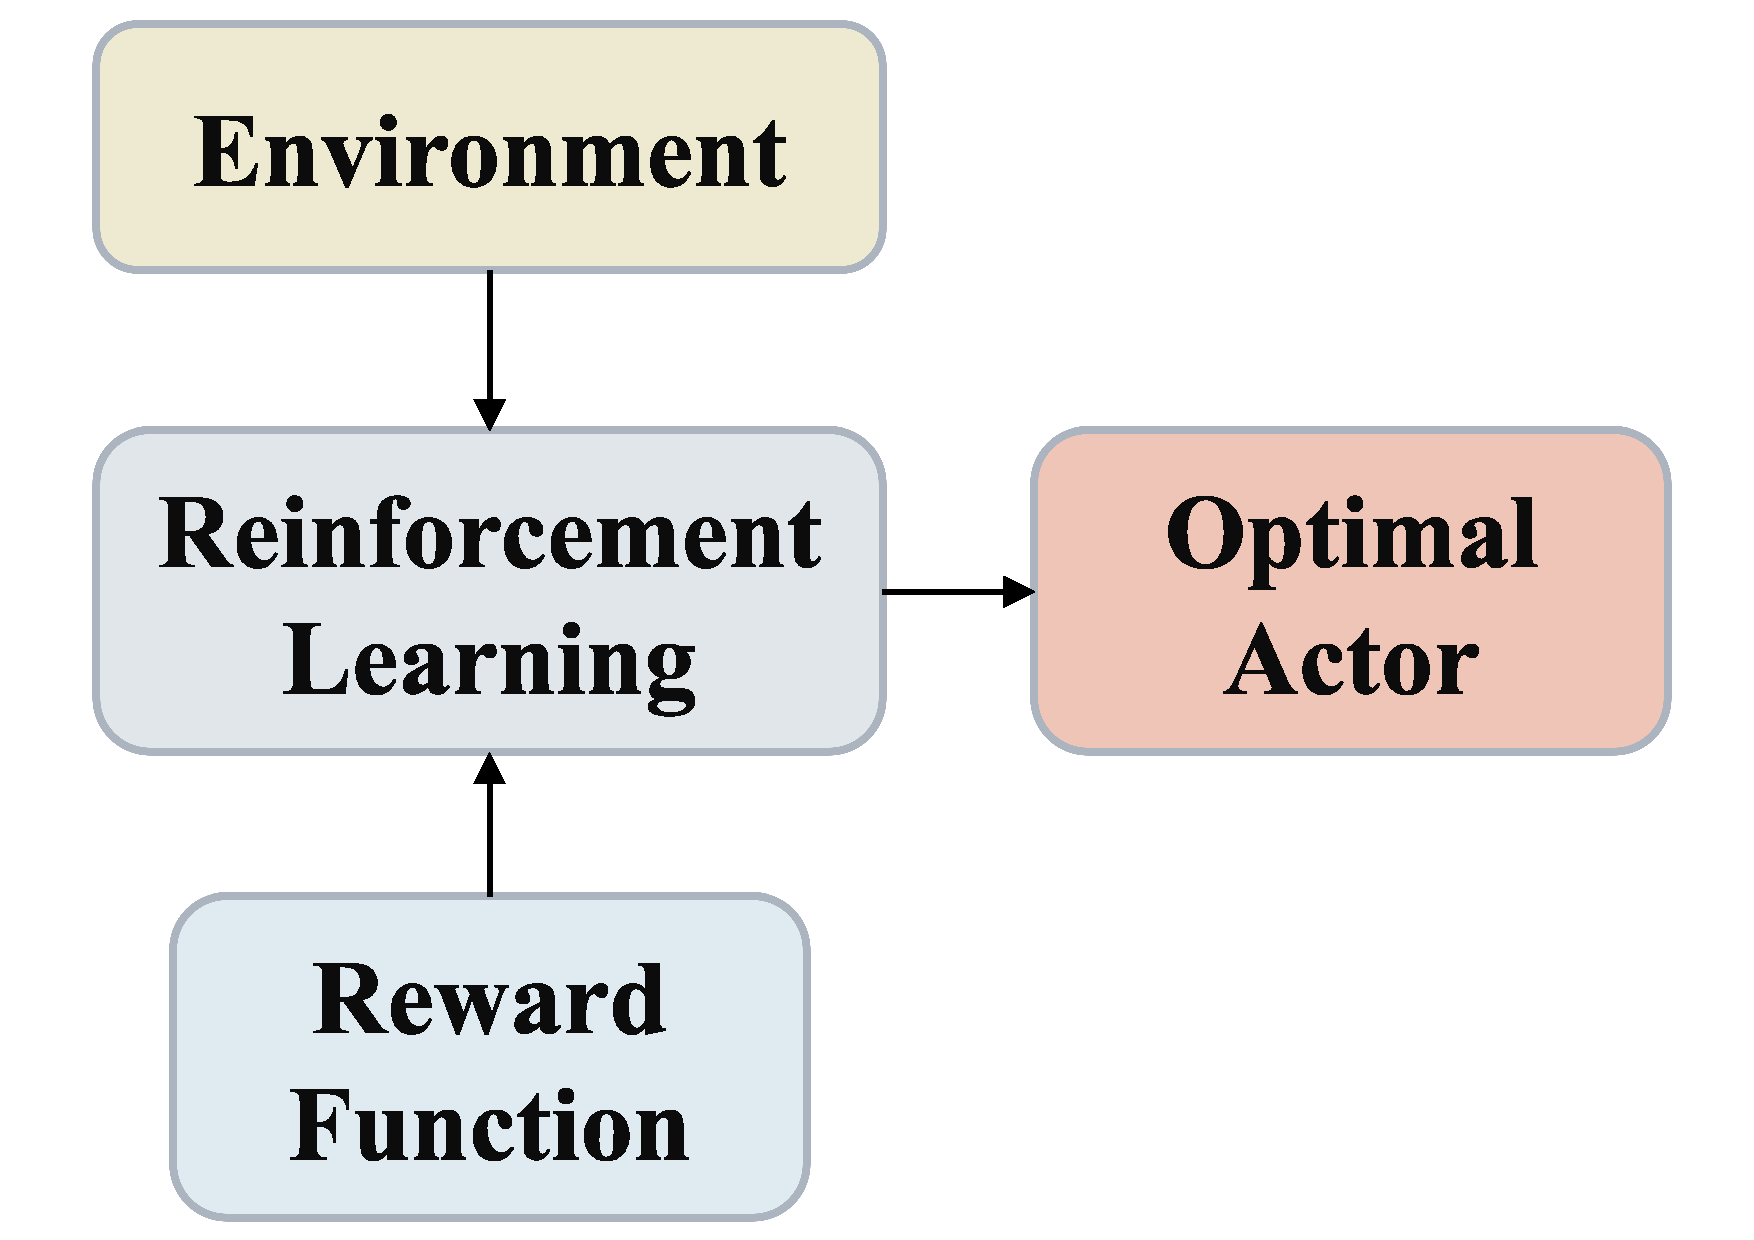
\includegraphics[width=\textwidth]{2_RL_mp.pdf}
		\caption{(a)}
		\label{fig:2_RL_mp}
	\end{subfigure}
	\hfill
	\begin{subfigure}{0.5\textwidth}
		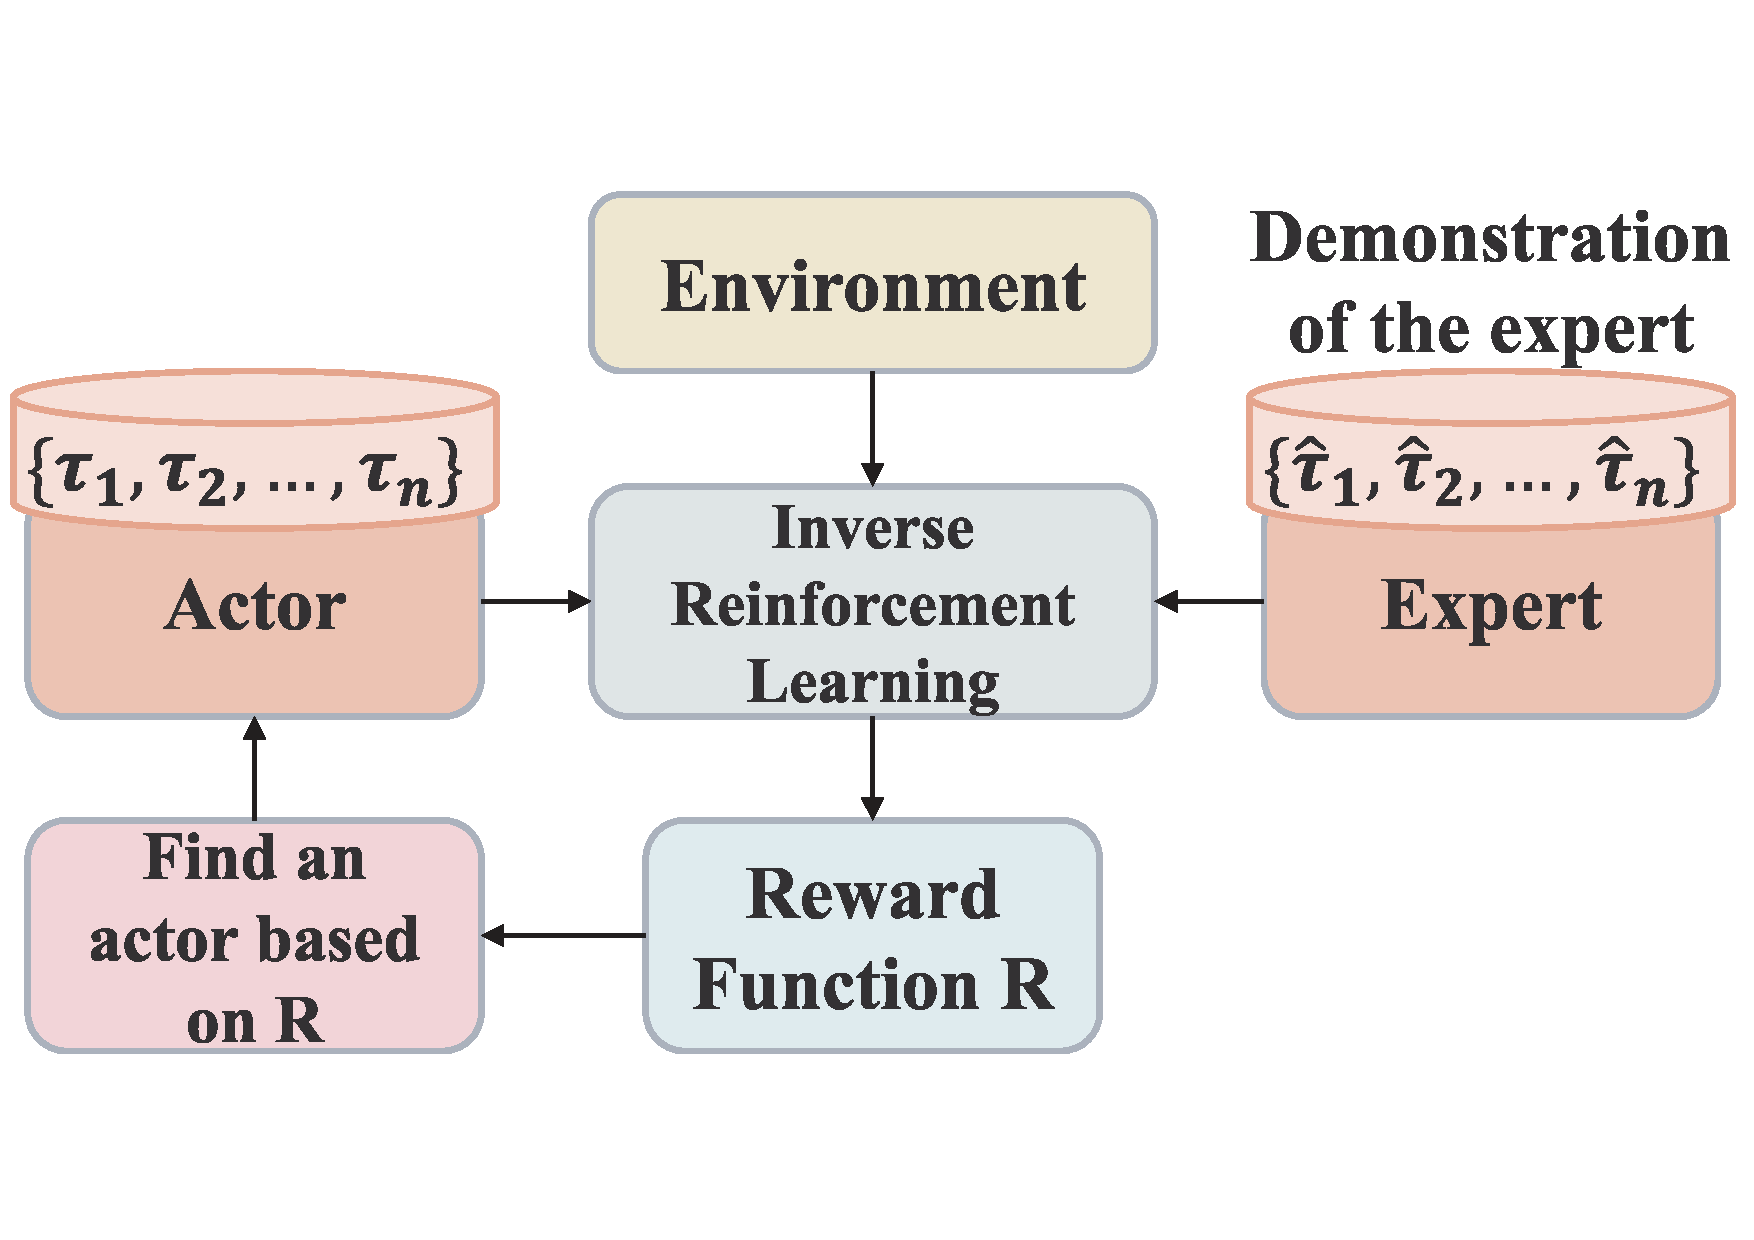
\includegraphics[width=\textwidth]{2_IRL_mp.pdf}
		\caption{(b)}
		\label{fig:2_IRL_mp}
	\end{subfigure}
	
	\caption[Reinforcement Learning vs Inverse Reinforcement Learning]{Description of (a) Reinforcement Learning and (b) Inverse Reinforcement Learning}
	Source: \textit{A survey on trajectory-prediction methods for autonomous driving} \cite{huang2022survey}
	\label{fig:2_RL_vs_IRL}
\end{figure}

\subsubsection{Inverse Reinforcement Learning (IRL)}
\label{subsubsec:2_irl_mp}

Usually, MDP assumes that the reward function is already provided. However, the driver’s behavior is always complicated such that manually specifying the weight of the reward function is inappropriate \cite{guan2018markov}. IRL learns the reward function according to the expert demonstration (trajectory) to generate the corresponding optimal driving policy as shown in Figure \ref{fig:2_IRL_mp}, in contrast to the RL approach where we must know the weight of a reward associated to a specific action. These IRL methods may be divided into groups: maximum margin-based and maximum entropy-based methods, where the main difference is the way of learning the weights of the reward function. \\
 
Maximum margin-based methods optimize the reward function weights by minimizing the feature expectations between the expert demonstration and the predicted trajectory. For example, \cite{silver2013learning} use maximum margin planning framework to learn reward functions and learn driving maneuvers for \acp{ADS}. However, most margin-based methods are ambiguous in the matching of feature expectations, because some degeneracies can also satisfy the optimal policy of expert demonstration. \\

On the other hand, Maximum entropy-based methods are more popular because they can use multiple reward functions to explain the ambiguity of experts's behavior \cite{aghasadeghi2011maximum}, most of which are based on linear mapping and can be formulated as:

\begin{equation}
\begin{aligned}
r(\Phi(s))=\theta^{\top} \Phi(s)
\end{aligned}
\end{equation}

where $r$ is the approximation of reward function; $\Phi$ is a function to output the features of the state $s$, and the weight $\theta$ will be acquired by training. Several works apply maximum entropy-based IRL (MaxEnt-IRL) to behavior prediction for AVs. In \cite{herman2015inverse}, using MaxEnt-IRL acceptability-dependent behavior models are learned from expert's trajectories to generate the stochastic behavior, then the optimum behavior model is chosen by maximizing the social acceptability. \cite{sharifzadeh2016learning} leverage IRL with Deep Q-Networks (DQN) to extract the rewards with large state spaces. In \cite{sun2018probabilistic}, interaction-related factors are considered to accomplish probabilistic prediction for \acp{ADS}. The distribution for future trajectories is formulated by driving maneuvers. Based on the decision-making mechanism, reward functions are learned using a polynomial trajectory sampler with discrete latent driving intentions in \cite{huang2021driving}.

\subsubsection{Generative Adversarial Imitation Learning (GAIL)}
\label{subsubsec:2_gail_mp}

Instead of learning the reward function from experts’ demonstration with IRL, Generative Adversarial Imitation Learning (GAIL) \cite{torabi2018generative} uses the method of GAN to do imitation learning in RL. GAIL directly extracts policies from data where, as proposed by a \ac{GAN} \cite{goodfellow2020generative}, the core idea of GAIL is that the generator generates a trajectory similar to the expert trajectory as much as possible, and the discriminator tries to judge whether it is an expert trajectory as much as possible. Many articles use GAIL to complete trajectory prediction for \ac{AD}. \cite{kuefler2017imitating} extend GAIL to the optimization of RNN to demonstrate human driver behaviors, and policies and actions are evaluated by the discriminator. In \cite{bhattacharyya2022modeling}, a parameter-sharing extension of GAIL is proposed to model the interaction between multi-agent and can provide agents with domain-specific knowledge. To overcome the shortcomings of GAIL, which only models the next state using the current state, \cite{choi2021trajgail} propose a method combining a partially observable Markov decision process (POMDP) within the GAIL framework, and the model is trained using the reward function from the discriminator.

\subsubsection{Deep Inverse Reinforcement Learning (DIRL)}
\label{subsubsec:2_dirl_mp}

Since the prediction problem in \ac{AD} is usually non-linear, i.e. the agent does not traverse in a straight path, it is necessary to use non-linear mapping for generalizable function approximations. In that sense, Deep Inverse Reinforcement Learning (DIRL) is proposed \cite{wulfmeier2015maximum} to approximate complex and nonlinear reward functions, which can be expressed as:

\begin{equation}
\begin{aligned}
r(\Phi(s))=f(\theta, \Phi(s))
\end{aligned}
\end{equation}

where $f$ is a nonlinear function. Some DIRL methods take historical trajectories as input. \cite{you2019advanced} consider the driving style and the road geometry, where the authors first use RL to design MDP, then learn the optimal driving policy from IRL, and use the deep neural network (DNN) to approximate the reward function. In \cite{fernando2020deep}, trajectories of traffic participants are encoded by LSTM and the reward network is learned by FCN. Currently, more DIRL-based methods directly use raw perception data. \cite{wulfmeier2017large} apply FCN for mapping the lidar data to traversability maps. The network is pre-trained to regress to a manual prior cost map and the initialize weights will be fine-tuned by the maximum entropy DIRL network. \cite{zhu2020off} use RL ConvNet and state visiting frequency (SVF) ConvNet to encode the vehicle’s kinematics and obtain the weight of the reward function by back-propagating the loss gradient \cite{wulfmeier2016watch} between expert SVF from expert demonstration and policy SVF from lidar data.

\subsection{Deep Learning based Motion Prediction}
\label{sec:2_dl_based_mp}

The Deep Learning (DL) methods are the last type of \ac{MP} methods covered in Chapter since its different approaches are, by far, the most used at this moment in the field of \ac{MP} in \ac{AD} to predict the future trajectory of traffic participants., being this thesis focused in these particular methods. Most traditional predictions methods \cite{huang2022survey}, which usually only consider physics-related factors (like the velocity and acceleration of the target vehicle that is going to be predicted) and road-related factors (prediction as close as possible to the road centerline), are only suitable for short-time prediction tasks \cite{huang2022survey} and simple traffic scenarios, such as constant velocity (CV) in a highway or a curve (Constant Turn Rate Velocity, CTRV) where a single path is allowed, i.e. multiple choices computation are not required. Recently, MP methods based on DL have become increasingly popular since they are able not only to take into account these above-mentioned factors but also consider interaction-related factors (like agent-agent \cite{gupta2018social}, agent-map \cite{casas2018intentnet} and map-map \cite{liang2020learning}) in such a way the algorithm can adapt to more complex traffic scenarios (intersections, sudden breaks and accelerations, etc.). It must be consider that multimodal, specially in the field of vehicle motion prediction, does not refer necessarily to different directions (e.g. turn to the left, turn to the right, continue forward in an intersection), but it may refer to different predictions in the same direction that model a sudden positive or negative acceleration, so as to imitate a realistic human behaviour in complex situations. As expected, neither classical nor machine learning (ML) methods can model these situations \cite{huang2022survey}. \\

\begin{figure}[h]
	\centering
	% trim={left bottom right top}
	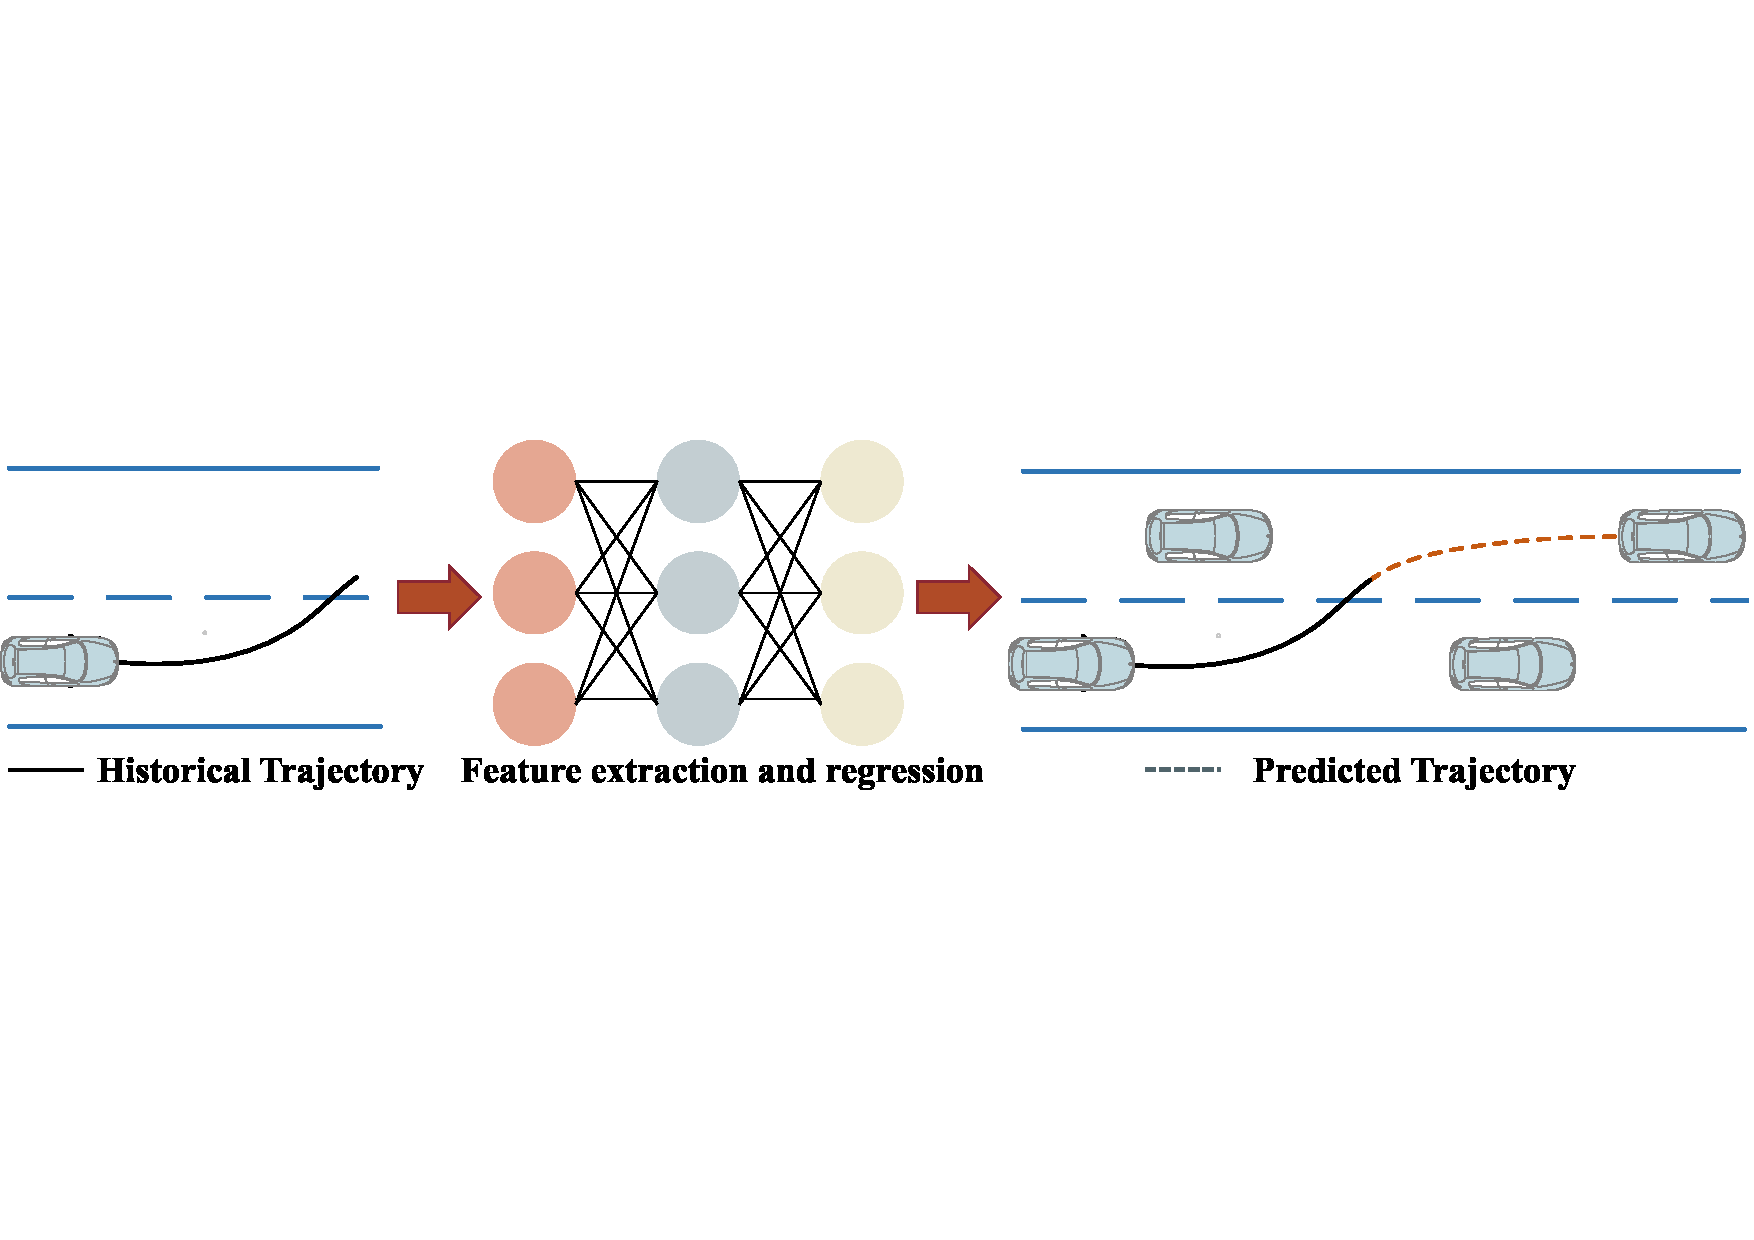
\includegraphics[trim={0 7cm 0 7cm}, width=\linewidth]{2_DL_methods_mp.pdf}
	\caption{Deep Learning methods applied in Motion Prediction}
	Source: \textit{A survey on trajectory-prediction methods for autonomous driving} \cite{huang2022survey}
	\label{fig:2_DL_example_mp}
\end{figure}

The main DL-based approaches are: \acp{CNN}, Recurrent Neural Networks (RNNs), \acp{GAN}, Attention mechanisms and \acp{GNN}. Figure \ref{fig:2_DL_example_mp} illustrates the main idea of using \ac{DL} to predict the future trajectories of the agents. Since this thesis is focused on developing efficient and accurate \ac{DL}-based \ac{MP} models in the field of \ac{AD}, the theoretical explanation of these different neural networks used in our pipelines will be explained in the Chapter 3 \ref{cha:theoretical_background} along with some physics-based models theory to fully-understand the proposed models. The input is represented by, at least, the physics-factors of the corresponding, though road-factors and interaction-factors are present in most \ac{DL} algorithms. Then, a neural network extracts the most important features and outputs a future trajectory according to the training process in a supervised way. \\

In order to classify \ac{DL} based \ac{MP} methods, we can identify the different factors (physics, interaction and road) and determine which type of neural network is employed to extract features of the corresponding input. In the literature we mainly distinguish the following inputs and outputs: Motion history (physics-based factors), Social information (interaction-based factors), Map information (road-relared factors), how the model returns the output trajectory and its corresponding distribution. Table \ref{table:2_dl_related_work_mp} summarizes several SOTA methods.

\begin{table}[h!]
	\centering
	\caption[Main state-of-the-art Deep Learning methods for Motion Prediction]{Main state-of-the-art Deep Learning methods for Motion Prediction. Main categories are Encoder (splitted into motion history, social info (agent interactions) and map info (physical information)), Decoder, Output representation and Distribution over future trajectories}
	\begin{adjustbox}{max width=\textwidth}
		\begin{tabular}{l |ccc|c|c|c}
			\textbf{Method}	&	& \textbf{Encoder}	&	& \textbf{Decoder}	& \textbf{Output}  & \textbf{Trajectory Distribution}	\\
			& Motion history	& Social info	& Map info	&	&	&	\\
			\midrule
			\midrule
			SocialLSTM~\cite{alahi2016social}	& LSTM	& spatial pooling	& --	& LSTM	& states	& samples	\\
			SocialGan~\cite{gupta2018social}	& LSTM	& maxpool	& --	& LSTM	& states	& samples	\\
			Jean~\cite{mercat2020multi}	& LSTM	& attention	& --	& LSTM	& states	& GMM	\\
			TNT~\cite{zhao2021tnt}	& polyline	& maxpool, attention	& polyline	& MLP	& states	& weighted set	\\
			LaneGCN~\cite{liang2020learning}	& 1D-conv	& GNN	& GNN	& MLP	& states	& weighted set	\\
			WIMP~\cite{khandelwal2020if}	& LSTM	& GNN+attention	& polyline	& LSTM	& states	& GMM	\\
			VectorNet~\cite{gao2020vectornet}	& polyline	& maxpool, attention	& polyline	& MLP	& states	& unimodal	\\
			SceneTransformer~\cite{ngiam2022scene}	& attention	& attention	& polyline	& attention	& states	& weighted set	\\
			HOME~\cite{gilles2021home}	& raster	& attention	& raster	& conv	& states	& heatmap	\\
			GOHOME~\cite{gilles2022gohome}	& 1D-conv+GRU	& GNN	& GNN	& MLP	& states	& heatmap	\\
			MP3~\cite{casas2021mp3}	& raster	& conv	& raster	& conv	& cost function	& weighted samples	\\
			CoverNet~\cite{phan2020covernet}	& raster	& conv	& raster	& lookup	& states	& GMM w/ dyn. anch.	\\
			DESIRE~\cite{lee2017desire}	& GRU	& spatial pooling	& raster	& GRU	& states	& samples	\\
			MFP~\cite{tang2019multiple}	& GRU	& RNNs+attention	& raster	& GRU	& states	& samples	\\
			MANTRA~\cite{marchetti2020mantra}	& GRU	& --	& raster	& GRU	& states	& samples	\\
			PRANK~\cite{biktairov2020prank}	& raster	& conv	& raster	& lookup	& states	& weighted set	\\
			IntentNet~\cite{casas2018intentnet}	& raster	& conv	& raster	& conv	& states	& unimodal	\\
			Multimodal~\cite{cui2019multimodal}	& raster	& conv	& raster	& conv	& states	& weighted set	\\
			MultiPath~\cite{chai2019multipath}	& raster	& conv	& raster	& MLP	& states	& GMM w/ static anchors	\\
			MultiPath++~\cite{varadarajan2022multipath++}	& LSTM	& RNNs+maxpool	& polyline	& MLP	& control poly	& GMM	\\
			PLOP~\cite{buhet2021plop}	& LSTM	& conv	& raster	& MLP	& state poly	& GMM	\\
			Trajectron++\cite{salzmann2020trajectron++}	& LSTM	& RNNs+attention	& raster	& GRU	& controls	& GMM	\\
			CRAT-PRED\cite{schmidt2022crat}	& LSTM	& GNN+attention	& --	& MLP	& states	& weighted set	\\
			R2P2~\cite{rhinehart2018r2p2}	& GRU	& --	& polyline	& GRU	& motion	& samples	\\
			DKM~\cite{cui2020deep}	& raster	& conv	& raster	& conv	& controls	& weighted set	\\
		\end{tabular}
		\label{table:2_dl_related_work_mp}
	\end{adjustbox}
\end{table}

\begin{itemize}
	\item \textbf{Motion history}: Most methods encode the sequence of past observed states using 1D-convolution \cite{liang2020learning} \cite{mercat2020multi}, able to model spatial information, or via a recurrent net \cite{alahi2016social} (LSTM, GRU), which are more useful to handle temporal information. Other methods that use a raster version of the whole scenario represent the agent states rendered as a stack of binary mask images depicting agent oriented bounding boxes \cite{gilles2021home}. On the other hand, other approaches encode the past history of the agents in a similar way to the road components of the scene given a set of vectors or polylines \cite{zhao2021tnt, gao2020vectornet} that can model the high-order interactions among all components, or even employing attention to combine features across road elements and agent interactions \cite{ngiam2022scene}.
	
	\item \textbf{Social information}: In complex scenarios, motion history encoding of a particular target agent is not sufficient to represent the latent space of the traffic situation, but the algorithm must deal with a dynamic set of neighbouring agents around the target agent. Common techniques are aggregating neighbour motion history with a permutation-invariant set operator: soft attention \cite{ngiam2022scene}, a combination of soft attention and RNN \cite{varadarajan2022multipath++} / GNN \cite{schmidt2022crat} or social pooling \cite{alahi2016social, gupta2018social}. Raster based approaches rely on 2D convolutions \cite{chai2019multipath} \cite{casas2021mp3} over the spatial grid to implicitly capture agent interactions in such a way long-term interactions are dependent on the neural network receptive fields.
	
	\item \textbf{Map information}: High-fidelity maps \cite{can2022maps} have been widely adopted to provide offline information (also known as physical context) to complement the online information provided by the sensor suite of the vehicle and its corresponding algorithms. Recent learning-based approaches \cite{mahjourian2022occupancy, casas2018intentnet, ivanovic2021heterogeneous}, which present the benefit of having probabilistic interpretations of different behaviour hypotheses, require to build a representation to encode the trajectory and map information. Map information is probably the feature with the clearest dichotomy: raster vs vector treatment. The raster approach encodes the world around the particular target agent as a stack of images (generally from a top-down orthographic view, also known as Bird's Eye View). This world encoding may include from agent state history, agent interactions and usually the road configuration, integrated all this different-sources information as a multi-channel image \cite{gilles2021home}, in such a way the user can use an off-the-shelf Convolutional Neural Network (CNN) based pipeline in order to leverage this powerful information. Nevertheless, this representation has several downsides: constrained field of view, difficulty in modeling long-range interactions and even difficulty in representing continuous physical states due to the inherent world to image (pixel) discretization. On the other hand, the polyline approach may describe curves, such as lanes, boundaries, intersections and crosswalks, as piecewise linear segments, which usually represents a more compact and efficient representation than using CNNs due to the sparse nature of road networks. Some state-of-the-art algorithms not only describe the world around a particular agent as a set-of-polylines \cite{khandelwal2020if} \cite{zhao2021tnt} in an agent-centric coordinate system, but they also leverage the road network connectivity structure \cite{liang2020learning} \cite{zeng2021lanercnn} treating road lanes as a set of nodes (waypoints) and edges (connections between waypoints) in a graph neural network so as to include the topological and semantic information of the map.
	
	\item \textbf{Decoder}: Pioneering works of DL based MP usually adopt the autoencoder architecture, where the decoder is often represented by a recurrent network (GRU, LSTM, etc., specially designed to handle temporal information) to generate future trajectories in an autoregressive way, or by CNNs \cite{gilles2021home} \cite{gilles2022gohome} / MLP \cite{liang2020learning} \cite{schmidt2022crat} using the non-autoregressive strategy. The method may use an autoregressive strategy where the pipeline generates tokens (in this case, positions or relative displacements) in a sequential manner, in such a way the new output is dependent on the previously generated output, whilst MLP \cite{schmidt2022crat}, CNN \cite{gilles2021home} or transformer \cite{ngiam2022scene} based strategies usually follow a non-autoregressive strategy, where from a latent space the whole future trajectory is predicted.
	
	\item \textbf{Output}: The most popular model output representation is a sequence of states (absolute positions) or state differences (relative displacements for any dimension considered). The spacetime trajectory may be intrinsically represented as a continous polynomial representation or a sequence of sample points. Other works \cite{gilles2021home} \cite{gilles2022gohome} first predict a heatmap and then decode the corresponding output trajectories after sampling points from the heatmap, whilst \cite{casas2021mp3} \cite{zeng2019end} learn a cost function evaluator of trajectories that are enumerated heuristically instead of being generated by a learned model. 
	
	\item \textbf{Trajectory Distribution}: The choice of output trajectory distributions has several approaches on downstream applications. Regardless the agent to be predicted is described as a (non-)holonomic \cite{triggs1993motion} platform, an intrinsic property of the motion prediction problem is that the agent must follow one of a diverse set of possible future trajectories. A popular choice to represent a multimodal prediction are Gaussian Mixture Models (GMMs) due to their compact parameterized form, where mode collapse (associated frequently to GMMs) is addressed through the use of trajectory anchors \cite{chai2019multipath} or training  tricks \cite{cui2019multimodal}. Other approaches model a discrete distribution via a collection of trajectory samples extracted from a latent space and decoded by the model \cite{rhinehart2018r2p2} or over a set of trajectories (fixed or a priori learned) \cite{liang2020learning}.
\end{itemize}

\section{Summary}

In order to finish this Chapter, we perform a brief comparison between the different methods (Physics-based, Classic ML, Reinforcement Learning and \ac{DL}) in terms of accuracy, prediction horizon, computation cost and applications in the \ac{AD} field. 

\begin{table}[h!]
	\centering
	\caption[Summary of Motion Prediction methods features]{Summary of Motion Prediction methods features. Short-term and long-term characterize prediction horizons of no more than 1-s and no less than 3-s, respectively.}
\begin{adjustbox}{max width=\textwidth}
%\begin{tabular}{|P|P|P|P|P|}
\begin{tabular}{|c|c|c|c|c|}
	\hline
	Methods & Accuracy & $\begin{array}{l}\text { Prediction } \\
		\text { Horizon }\end{array}$ & $\begin{array}{l}\text { Computation } \\
		\text { Cost }\end{array}$ & Applications \\ \hline 
	
	Physics-based & $\begin{array}{l}\text { High in short-term prediction,  } \\
		\text { low in other prediction horizon }\end{array}$ & Short & Small & Colision risk analysis \\ \hline
	 $\begin{array}{l}\text { Classic Machine } \\
		\text { Learning-based }\end{array}$ & $\begin{array}{l}\text { Good at recognizing maneuvers but } \\
		\text { generalization ability is poor }\end{array}$ & Medium & Medium & Maneuver recognition \\ \hline
	
	 Deep Learning-based & High in considering some factors & Long & $\begin{array}{l}\text { Relatively } \\
		\text { high }\end{array}$ & $\begin{array}{l}\text { More and more applied } \\
		\text { in real-world }\end{array}$ \\ \hline
	
	 $\begin{array}{l}\text { Reinforcement } \\
		\text { Learning-based }\end{array}$ & $\begin{array}{l}\text { Relatively high, prediction methods  } \\
		\text { are relatively few }\end{array}$ & Long & High & More applied in planning \\
	\hline
\end{tabular}
\label{table:2_summary_mp_methods}
\end{adjustbox}
\end{table}

\begin{itemize}
	\item Physics-Based Methods are suitable for the movement of vehicles, which can be accurately described by kinematics or dynamics models. Given a suitable physics model, these methods can be applied to a variety of scenarios at small computational cost and in a short time but without training. However, the prediction results based on such models heavily depends on the inputs and the model selection. The inputs are closely related to human or machine drivers, influenced by the driving environment or the interactions with other participants. Therefore, without the capability to describe such factors, physics-based models are limited to short-term prediction and in static scenes. Because of its simplicity and fast response, these methods can be easily used in real applications for \acp{ADS}, such as collision risk analysis.
	\item Classic Machine Learning-Based Methods, compared with physics-based methods, are able to consider more factors and its accuracy is relatively high with a longer prediction length at a higher computing cost. Most of these methods are maneuver-based methods, which predicts the trajectory with the maneuver known as a prior. However, vehicle maneuvers of human drivers are usually diverse and vary greatly in different scenarios such that the generalization ability of is poor. In real applications for AVs, such methods are used in scenarios such as lane change studies, leveraging their advantages in maneuver recognition.
	\item Reinforcement Learning-Based Methods imitate the human decision-making process and obtain the reward function through learning the expert demonstration to generate the corresponding optimal driving policy. They can continuously evolve through learning and adapt to complex environments and long prediction horizons. Such methods probably generate higher accuracy trajectories than deep learningmethods in a longer time domain. However, most of these methods are typically computationally expensive in their recovery of an expert cost function and require long training times. In real applications for AVs, reinforcement learning-based trajectory prediction methods are more applied to trajectory planning, taking its advantages in the decision-making process.
	\item Deep Learning-Based Methods can perform accurate predictions in a longer time horizon with respect to traditional methods that are only suitable for simple scenes and short-term prediction. By means of powerful neural networks, such as RNNs, CNNs, GANs, Attention mechanisms or GNNs for feature extraction, physics-related, interaction-related and road-related factors are processed as inputs to the model. Furthermore, they can adapt to more complex environments and a longer prediction horizon. \ac{DL}-based methods require to use a large amount of data for training. Besides, with the increase of consideration factors and the increase of the number of network layers, the computing costs and time increases sharply. Such methods can naturally generate multi-modal trajectories, which is consistent with the diversity of vehicles’ maneuvers. In real applications for AVs, it is necessary to reach a balance between calculation time and model complexity to ensure the real-time performance and safety of AVs. At present, more and more real-world trials use thesemethods to predict thefuture trajectory of traffic participants.
\end{itemize}	
	
As observed in Table \ref{table:2_summary_mp_methods} and discussed in this section summarizing the different \ac{MP} algorithms, we focus this thesis on \ac{DL} methods since they are the most suitable methods for long-term prediction with a relatively high computation cost, specially focusing on the ability of extracting and combining the latent spaces of the different inputs by means of \ac{SOTA} algorithms.